\documentclass[journal]{IEEEtran}

\ifCLASSINFOpdf
  % \usepackage[pdftex]{graphicx}
  % declare the path(s) where your graphic files are
  % \graphicspath{{../pdf/}{../jpeg/}}
  % and their extensions so you won't have to specify these with
  % every instance of \includegraphics
  % \DeclareGraphicsExtensions{.pdf,.jpeg,.png}
\else
  % or other class option (dvipsone, dvipdf, if not using dvips). graphicx
  % will default to the driver specified in the system graphics.cfg if no
  % driver is specified.
  % \usepackage[dvips]{graphicx}
  % declare the path(s) where your graphic files are
  % \graphicspath{{../eps/}}
  % and their extensions so you won't have to specify these with
  % every instance of \includegraphics
  % \DeclareGraphicsExtensions{.eps}
\fi

\usepackage{url}
\usepackage{amsmath,amssymb}
\usepackage{float}
\usepackage{graphicx,subfigure}
\usepackage{color}
\usepackage[colorlinks=true,linkcolor=black]{hyperref}
\usepackage{breakurl}
\usepackage{cite}
\usepackage[ruled,linesnumbered]{algorithm2e}
\usepackage{ amssymb }
\usepackage{mathrsfs }
\usepackage{enumitem} 
\usepackage{romannum}
\usepackage{hyperref}
\usepackage{amsthm}
\hypersetup{colorlinks,linkcolor={black},citecolor={black},urlcolor={red}}  


\newcommand{\minmax}{$\min\max$}
\newcommand{\pcomment}{\textcolor{blue}}
\newcommand{\ie}{\emph{i.e.,}}

\newcommand{\tabincell}[2]{\begin{tabular}{@{}#1@{}}#2\end{tabular}}


\DeclareMathOperator{\Tr}{tr}
\newcommand{\minimize}{minimize}

\newtheorem{theorem}{Theorem}
\newtheorem{lemma}{Lemma}
\newtheorem{definition}{Definition}
\newtheorem{problem}{Problem}


\begin{document}

\title{Computational Techniques for Efficient Active Target Tracking with State-Dependent Noise}

\author{Zhongshun Zhang and Pratap Tokekar% <-this % stops a space
\thanks{The authors are with the Department of Electrical \& Computer Engineering, Virginia Tech, USA. \texttt{\small \{zszhang,tokekar\}@vt.edu}.}%
\thanks{This material is based upon work supported by the National Science Foundation under Grant \#1566247.}}

\maketitle

\begin{abstract}
We study the problem of devising a closed-loop strategy to control the position of a robot that is tracking a possibly moving target. The robot obtains noisy measurements of the target's position. The measurement noise depends on the relative states of the robot and the target. We consider scenarios where the measurement values are chosen by an adversary so as to maximize the estimation error. Furthermore, the target may be actively evading the robot. Our main contribution is to devise a closed-loop control policy for state-dependent target tracking that plans for a sequence of control actions, instead of acting greedily. We seek to minimize the maximum uncertainty (trace of the posterior covariance matrix) over all possible measurement values. We exploit the structural properties of a Kalman Filter to build a policy tree that is orders of magnitude smaller than naive enumeration while still preserving optimality guarantees. We show how to obtain even more computational savings by relaxing the optimality guarantees. The resulting algorithms are evaluated through simulations and experiments with real robots.
\end{abstract}

\IEEEpeerreviewmaketitle



\section{Introduction}
Tracking a moving, possibly adversarial target is a fundamental problem in robotics and has long been a subject of study~\cite{bar2004estimation,li2003survey,li2010survey,li2001survey,li2002survey,li2005survey}. Target tracking finds applications in many areas such as surveillance~\cite{rao1993fully}, telepresence~\cite{karnad2012modeling}, assisted living~\cite{montemerlo2002experiences}, and habitat monitoring~\cite{isler2015finding,tokekar2013tracking}. Target tracking refers to broadly two classes of problems: (i) estimating the position of the target using noisy sensor measurements; and (ii) actively controlling the sensor position to improve the performance of the estimator. The second problem is distinguished as \emph{active} target tracking and is the subject of study of this paper. 

One of the main challenges in tracking is that the target can be adversarial and actively  avoid tracking by moving away from the robot. Furthermore, the value of future measurement locations can be a function of the unknown target state. Take as example, a simple instance of estimating the unknown position of a stationary target where the measurement noise is a function of the distance between the robot and the target. If the true location of the target were known, the robot would always choose a control sequence that drives it closer to the target. Since, in practice, the true target location is unknown, we cannot determine such a control sequence exactly. A possible strategy, in this case, would be to plan with respect to the probability distribution of the target. However, the probability distribution itself will evolve as a function of the actual measurement values. This becomes even more challenging if the target is mobile. 

In this paper, we use an Extended Kalman Filter (EKF) to estimate the state of a moving target with a possibly state-dependent measurement model where the measurement noise is a function of the distance between the robot and the target. We formulate the active tracking problem as a minimax game.  When planning non-myopically (for multiple steps in the future), one can enumerate all possible future measurements in the form of a tree. In particular, a minimax tree can be used to find the optimal (in the minimax sense) control policy for actively tracking a target~\cite{tokekar2011active}. The size of the minimax tree grows exponentially with the time horizon. The tree can be pruned using alpha-beta pruning~\cite{russell2009artificial}. Our main contribution is to show how the properties of an EKF can be exploited to prune a larger number of nodes without losing optimality. In doing so, we extend the pruning techniques first proposed by Vitus et al.~\cite{vitus2012efficient} for linear systems with state independent noise. Using a minimax tree, we generalize these results to a system with state-dependent noise. Our pruning techniques allow us to trade-off the size of the tree (equivalently, computation time) with the optimality guarantees of the algorithm. We demonstrate this effect in simulations and proof-of-concept indoor and outdoor tracking experiments. We also show how the tree can be updated online, when the measurements received and/or the target motion is not adversarial.

The rest of the paper is organized as follows. We start with the related work in Section~\ref{sec:relwork}. The problem formulation is presented in Section~\ref{sec:probform}. Our main algorithm is presented in Section~\ref{sec:pruning2}. The pruning condition in different cases is discussed in Section \ref{sec:pruning2}. We validate the algorithm through simulations that are described in Section~\ref{sec:sims} and experiments on real robots reported in Section~\ref{sec:expt}. Finally, we conclude with a brief discussion of future work in Section~\ref{sec:conc}. 

A preliminary version of the paper first appeared in CDC 2016~\cite{zhang2016non} without the online execution algorithm, without the Gazebo simulations and without the experiments on the real robots.

\section{Related Work} \label{sec:relwork}
The target tracking problem has been studied in various settings. Bar-Shalom et al.~\cite{bar2004estimation} have presented many of the commonly-used estimation techniques in target tracking. The five-part survey by Li and Jilkov~\cite{li2003survey,li2010survey,li2001survey,li2002survey,li2005survey} covers commonly-used control and maneuvering techniques for active target tracking.  

Pursuit-evasion is a class of problems typically used to study adversarial target tracking~\cite{chung2011search}. Kolling and Carpin~\cite{kolling2010pursuit} study a pursuit-evasion problem on graphs that model the detection of intruders in complex indoor environments by robot teams.  A typical approach is to model the problem as a two-player non-cooperative zero-sum game and use Pontryagin’s minimum principle and the Bellman equation to find the optimal paths for the pursuer~\cite{bacsar1998dynamic,lewis1995optimal,bhattacharya2009existence,bhattacharya2009game}. These approaches typically assume noise-free sensing. Amongst pursuit-evasion works that explicitly address measurement noise are works by Vander Hook and Isler~\cite{vander2014pursuit} using noisy bearing sensors and Rote~\cite{rote2003pursuit} using imprecise target measurements. The latter employs a bounded uncertainty model for the measurement noise, whereas we consider additive Gaussian noise.

Willman~\cite{willman1969formal} studied the differential pursuit-evasion problem with state-independent Gaussian noise to the motion model as well as the measurement model. The author showed that the problem can be reduced to a deterministic one. Yaesh and Shaked~\cite{yaesh1992game} have shown the connection between the $H_{\infty}$ optimal estimation theory and adversarial target tracking. Zengin and Dogan~\cite{zengin2007real} have presented a real-time target tracking for autonomous UAVs in adversarial environments. More recently, Gu~\cite{gu2011game} proposed a minimax filter to estimate the state of an adversarial target using noisy measurements from a sensor network. Specifically, they modeled the estimation problem as a differential zero-sum game. Unlike these works, we use a minimax search tree to (non-myopically) plan for the control actions of the robot.

A search tree can provide optimal or near-optimal policies for target tracking. However, building a search tree can be computationally expensive especially for large-scale instances. The key is to effectively prune the tree to yield computational savings. Vitus et al.~\cite{vitus2012efficient} presented an algorithm that computes the optimal scheduling of measurements for a linear dynamical system. The goal is to track a linear dynamical system using a set of sensors such that one sensor can be activated at any time instance. The posterior covariance in estimating a linear system in a Kalman filter depends on the prior covariance and sensor variance but not on the future measurement values (unlike the case in non-linear systems). Thus, one can build a search tree enumerating all possible sensor selections and choosing the one that minimizes the final covariance. The main contribution of Vitus et al. is to present a pruning technique to reduce the size of the tree while still preserving optimality.

Atanasov et al.~\cite{atanasov2014information} extended this result to active target tracking with a single robot. A major contribution was to show that robot trajectories that are nearby in space can be pruned away (under certain conditions), leading to further computational savings. This was based on a linear system assumption. In this paper, we build on these works and make progress towards generalizing the solution for state-dependent observation systems.

%%%%%%%%%%make change
A major bottleneck for planning for state-dependent observation systems is that the future covariance is no longer independent of the actual measurement values. For example, an Extended Kalman Filter (EKF) is typically used in place of Kalman Filter for estimating non-linear systems. In an EKF, the state is linearized about the current state estimate after every measurement. The covariance update equations use the linearized models and as such will depend on the state estimate and the measurements. Thus, the search tree will have to include all possible measurement values and not just all possible measurement locations. Furthermore, finding an optimal path is no longer sufficient. Instead, one must find an optimal policy that prescribes the optimal set of actions for all possible measurements. We show how to use a minimax tree to find such an optimal policy while at the same time leveraging the computational savings that hold for the linear case.

%%%%%%%%%%%%%%%%%%%%%%%%%%%%%%%%%%%%%%%%%%%%%%%%%%%%%%%%%%%%%%%%%%%%%%%%%%%%%%%%
\section{Problem Formulation} \label{sec:probform}
We assume that the position of the robot is known accurately using onboard sensors (\emph{e.g.}, GPS, laser, IMU, cameras). The motion model of the robot is given by:
\begin{equation}
  \label{eq1}
  X_r(t+1)=f(X_r(t),u(t))
\end{equation}
where $X_r=[x_r(t), y_r(t)]^T\in\mathbb{R}^2$ is the position of robot and $u(t)\in \mathcal{U} $ is the control input at time $t$.\footnote{This result can be extended to 3D and other state spaces } $\mathcal{U} $ is a finite space of control inputs. We assume there are $n$ actions available as control inputs at any time:
$$\mathcal{U}_r(t)=\{u_{r1}(t),u_{r2}(t),\cdots, u_{rn}(t)\}.$$

The robot has a sensor that gets a measurement of the target's position. We assume that the target's motion model is given by:
\begin{equation}
  \label{eq2}
  X_o(t+1)=C_tX_o(t)+u_o(t)+v(t)
\end{equation}   
where, $ X_o(t)=[ x_o(t),  y_o(t)]^T   $ is the position of the target and $v(t)$ is the process noise drawn from a Gaussian distribution of known covariance.

The task of the robot is to track the target using its noisy measurements. The measurements, $Z(t)$, can be a function of the states of the target and the robot:
\begin{equation}
  \label{eq3}
  Z(t)= H(X_r(t)) X_o(t)  +\omega(X_r(t), X_o(t))
\end{equation}
The measurement noise, $\omega(\cdot)$, is drawn from a 2D zero-mean Gaussian distribution where the variance of each dimension is independent and given by $\delta_1^2 +\delta_2^2d(X_r(t),X_o(t))$. Here,
\leftline{$d(X_r(t),X_o(t))=$}
\begin{equation}
\left\{
\begin{aligned}
\mathcal{C},\qquad \qquad &\quad ||X_r(t)-X_o(t)||_2>\mathcal{B} \\ 
    \frac{\mathcal{C}||X_r(t)-X_o(t)||_2}{\mathcal{B}} , &\quad ||X_r(t)-X_o(t)||_2 \le \mathcal{B} \\  
\end{aligned}
\right.
\label{eqn:cov}
\end{equation}



When the true distance between the robot and target is within $\mathcal{B}$, we assume that measurement noise is proportional to the true distance. When the distance is greater than $\mathcal{B}$, the variance is assumed to be a constant with a maximum value of $\mathcal{C}$. 

The estimated position and the covariance matrix of the target at time $t$, $ \hat{X}_o(t)$ and  $\hat{\Sigma}_o(t)$, are given by the EKF. The uncertainty in the estimate of the target's position is measured by the trace of the covariance matrix. The goal of the robot is to reduce the uncertainty in the target's estimate. The goal of the adversary is to increase the uncertainty. There are two types of adversaries:
\begin{enumerate}
\item \textbf{Game against nature:} Here, ``nature'' acts as an adversary and generates the worst-case measurements, $z(t)$, for the robot. In general, the measurements will not be the worst-case ones. However, planning against this adversary will lead to a policy that is robust to possible outlier measurements.
\item \textbf{Game against an escaping target:} Here, the target actively chooses $v_o(t)$ to increase the estimation error. In our model, since the measurement noise is a function of the distance between the robot and the target, an adversarial target will choose to move away from the robot.
\end{enumerate}
The minimax tree strategy can be applied to either or both types of adversaries. Formally, the problem considered in this paper can be formally stated as follows.

\begin{problem} 
Given an initial robot position, $X_r(0)$, and an initial target estimate, $[\hat{X}_o(0), \hat{\Sigma}_o(0)]$, find a sequence of control laws for the robot, $\sigma=u_0, u_1,\cdots,  u_{T} \in \mathcal{U}^T$ from time $t=0$ to $t=T$ to minimize trace of the covariance in the target's estimate at time $t=T$. That is, 
\begin{equation}
  \label{eq5}
 \mathop{\text{minimize}}_{u_r(t)} \max_{u_o(t), z(t)}  \quad \text{tr}(\Sigma_T).
\end{equation}
such that,
 $$      \qquad  \Sigma_{t+1}=\rho_{{t+1}}(\Sigma_{t}),\quad t=0,1,\cdots, T-1 $$ 
where $\rho_{t}(\cdot)$ is the Kalman Riccati equation~\cite{kumar1986stochastic}. 
\label{prob:main}
\end{problem}

The Riccati equation~\cite{kumar1986stochastic}, $\rho(\cdot)$, maps the current covariance matrix $\hat\Sigma_k$, under a new measurement to the covariance matrix at the next time step,
\begin{align}
 \rho(\hat{\Sigma}_t)=&C_t\hat{\Sigma}_tC_t^T-C_t\hat{\Sigma}_tH_{t }^T(H_{t}\hat{\Sigma}_tH_{t}^T+\hat{\Sigma}_{w})^{-1}H_{t}\hat{\Sigma}_tC_t^T\notag\\
 &+\Sigma_v.  \label{eq6}
\end{align}
Here, $H_t$ is the linearized measurement model computed about ${X}_r(t)$ at time $t$.
% $$H_k=\left.\frac{\partial  h(x_r(k), x_o(k))}{\partial   x_o(k)}\right|_{x_o(k|k-1)}$$ 
$\Sigma_{w}$ is the covariance of the measurement noise given in Equations~(\ref{eq3})--(\ref{eqn:cov}). 

The true position of the target is unknown making it impossible to determine $\Sigma_{w}$ exactly. Consequently, we use an estimate of $\Sigma_{w}$ using the estimated  target's position, $\hat{X}_o(k)$. Therefore, the optimal solution for the problem defined will be a closed-loop policy that  maps the estimated target's position to the optimal control action for the robot.
%


%%%%%%%%%%%%%%%%%%%%%%%%%%%%%%%%%%%%%%%%%%%%%%%%%%%%%%%%%%%%%%%%%%%%%%%%%%%%%%%%

Earlier works~\cite{vitus2012efficient, atanasov2014information} solve a similar problem but with a linear Gaussian system. The linearity assumption makes the Riccati equation independent of the position of the target (known as the separation principle). Consequently, they show an open loop policy can determine the optimal control sequence for the robot. In our case, the optimal control policy will be a closed-loop one since the measurement noise is a function of the position of the target. However, this generalization comes at the expense of discretization of the set of possible target measurements. Specifically, we assume that the measurement at any time step is chosen from one of $m$ tuples of candidate measurements.\footnote{These $m$ candidate measurements can be obtained by, for example, sampling from the continuous distribution of zero mean sensor noise around the current estimate of the target.} That is,
$$z(t) \in \{z_1(t),z_2(t),\cdots, z_m(t)\}.$$
For example, we can choose $m$ candidate measurements from the data within 3 standard deviations of the mean value, which contain $99.7\%$ of the possible measurements. Figure~\ref{c2dGuassianfig} shows a discretized Gaussian distribution. 
\begin{figure}[H]
  \centering
  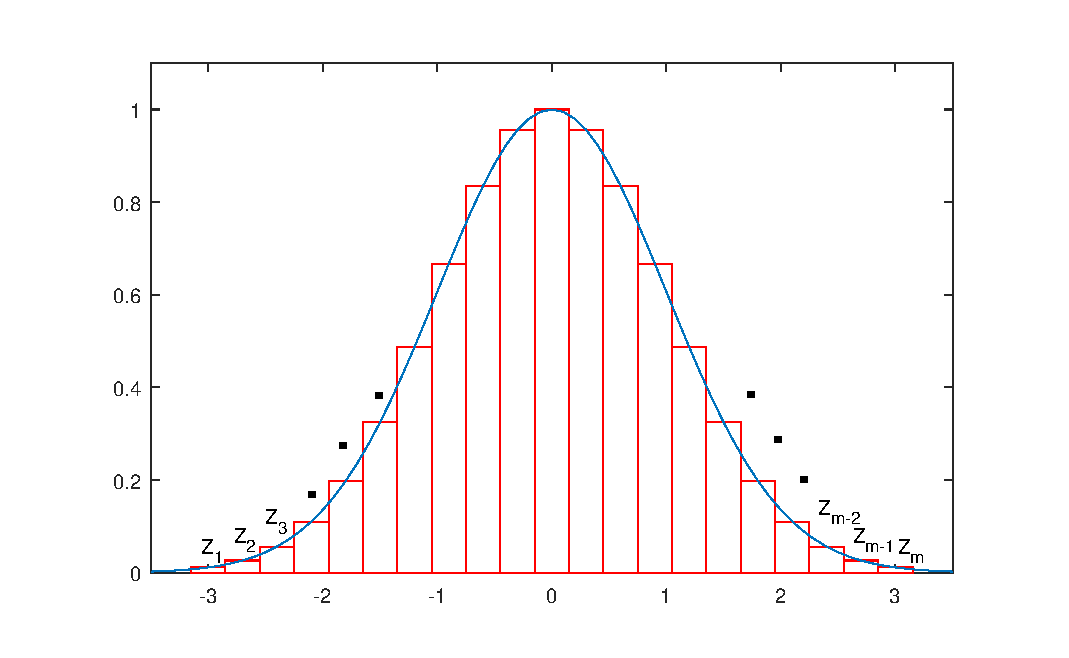
\includegraphics[height=3.5cm  ]{figs/c2dGuassian.eps}
  \caption{We discretize the set of candidate measurements using $m$ samples drawn from a Gaussian distribution.}
  \label{c2dGuassianfig}
\end{figure}

In the next section, we present the minimax tree strategy and various pruning techniques that allow us to efficiently find the optimal closed-loop policy for this problem.


\section{The minimax algorithm and pruning techniques} \label{sec:pruning2}


\begin{table*}[!htbp]
  \centering
\caption{Search Tree and Pruning Techniques for Various Models}
\label{table1}
\begin{center}
\begin{tabular}{|c|c|c|c|}
\hline
\textbf{Measurement Noise} & \textbf{\tabincell{c}{Target Motion}} & \textbf{Strategy} & \textbf{Pruning Algorithm}\\
\hline
State-independent & Known/Stationary & Search tree & Algebraic redundancy (Theorem~\ref{thm:fromvitus})\\
\hline
State-independent & Adversarial & \tabincell{c}{Minimax tree } & \tabincell{c}{Alpha-beta pruning, \\Algebraic redundancy (Theorem~\ref{thm:fromvitus})} \\
\hline
\tabincell{c}{State-dependent} & Known/Stationary & \tabincell{c}{Minimax tree }  & \tabincell{c}{Alpha pruning} \\
\hline
State-dependent & Adversarial & \tabincell{c}{Minimax tree } & \tabincell{c}{Alpha-beta pruning, \\Algebraic redundancy (Theorem~\ref{thm:main})} \\
\hline
\end{tabular}
\end{center}
\end{table*}


We model Problem~\ref{prob:main} as a sequential game\footnote{Note that, in practice, the robot and the target can move simultaneously.} played between the robot and an adversary. The robot executes a control action, takes a measurement of the target, the target moves to the new position, and the sequence repeats. Based on this, we generate a search tree to find the optimal policy. The adversary (\ie{} nature) chooses measurement noise and the target chooses actions at every step, whereas the robot chooses its own actions. By optimizing the minimax trace, the robot determines the best conservative policy.

\begin{figure}[h] 
  \centering
  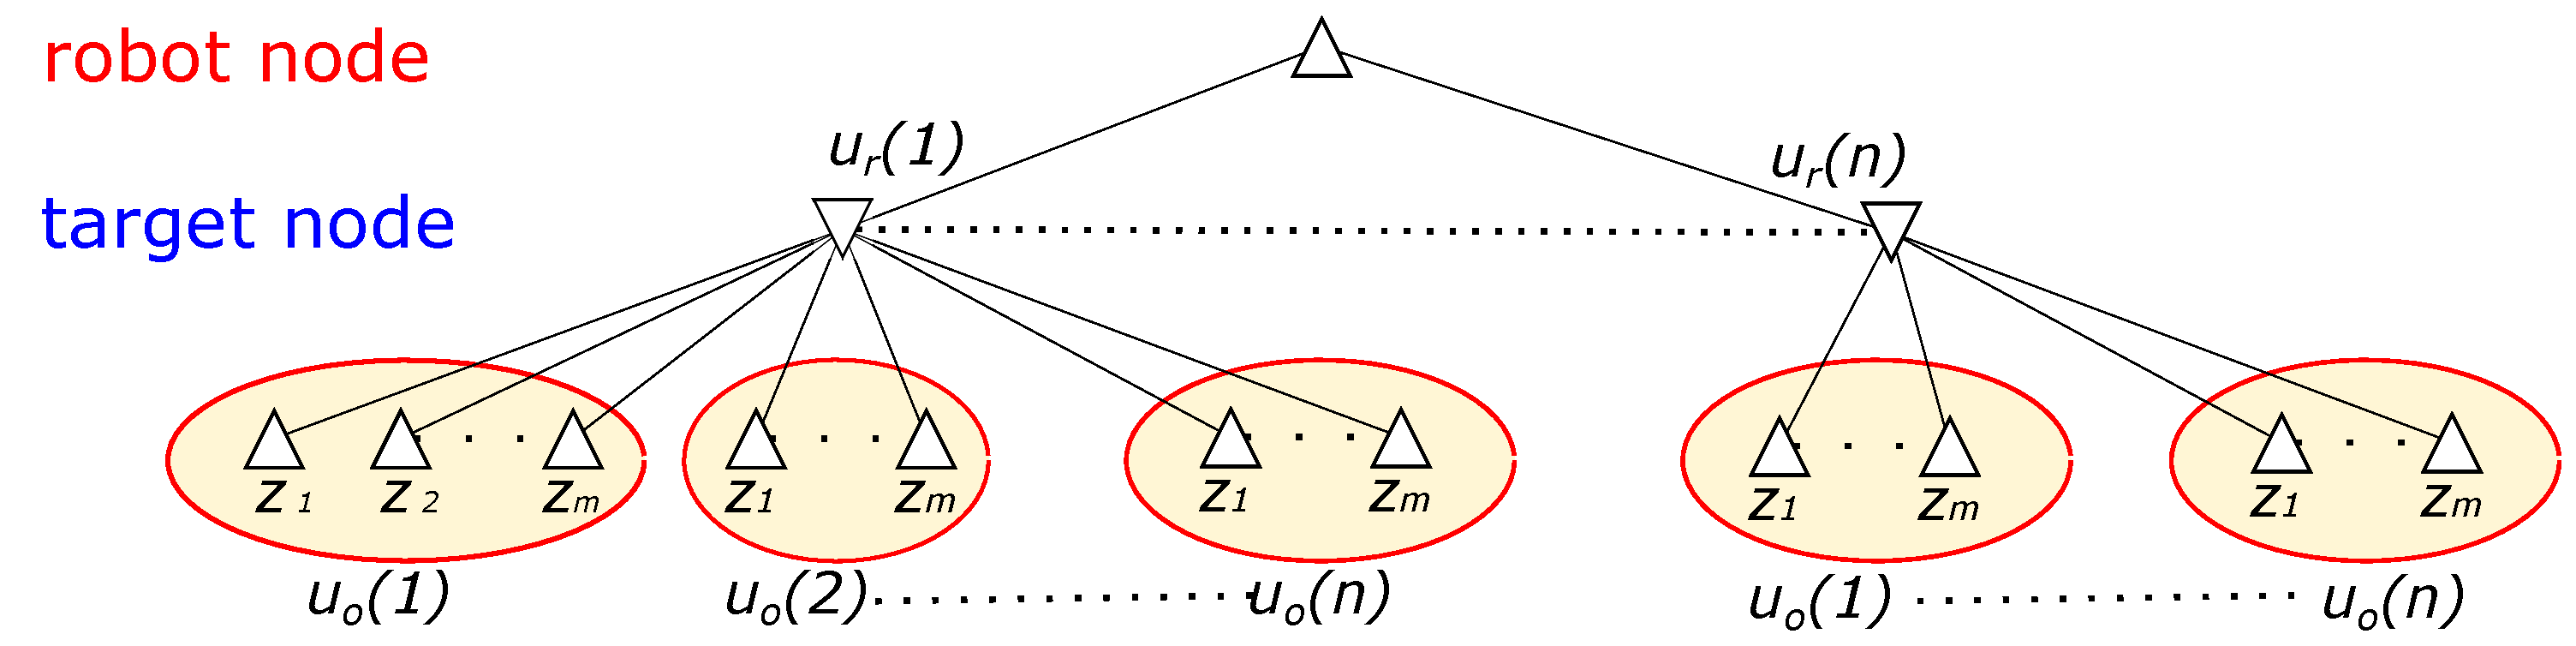
\includegraphics[width=0.9\columnwidth]{figs/MINMAX_tree_cases2.eps}
  \caption{One step minimax tree enumerates all the possible actions the robot and target as well as all candidate measurements. Each node in the tree stores the robot position and estimated target position.}
  \label{MINMAX_tree_case2}
\end{figure}

We find this optimal strategy by building a minimax tree. Figure~\ref{MINMAX_tree_case2} shows an example.  This tree enumerates all possible control laws for the robot and the target and all possible measurements that the robot can obtain. A node on the $k$th level of the tree stores the position of the robot, $X_r(k)$, the estimated position of the target, $\hat{X}_o(k)$, and the covariance matrix $\hat{\Sigma}_k$. Each node at an odd level has one branch per control action of the robot. We term these nodes as ``robot nodes.'' Each node at an even level has one branch per tuple of candidate measurement and candidate actions for the target. These nodes are termed as the ``target nodes.'' 

The robot's state and the target's estimate are updated appropriately along the control and measurement branches using the state transition equation (Equation~\ref{eq1}) and the EKF update equation, respectively. The minimax value is computed at the leaf nodes and is equal to the trace of the covariance matrix at that node. These values are propagated upwards to compute the optimal strategy. 

The full enumeration tree has a size exponential in the number of control actions, candidate measurements, and the planning horizon. We present three pruning strategies to reduce the size of the tree. The first two are based on existing alpha-beta pruning while the third one is a new contribution of this paper. Table~\ref{table1} gives the summary of all pruning techniques.

\begin{figure*}[h] 
  \centering
  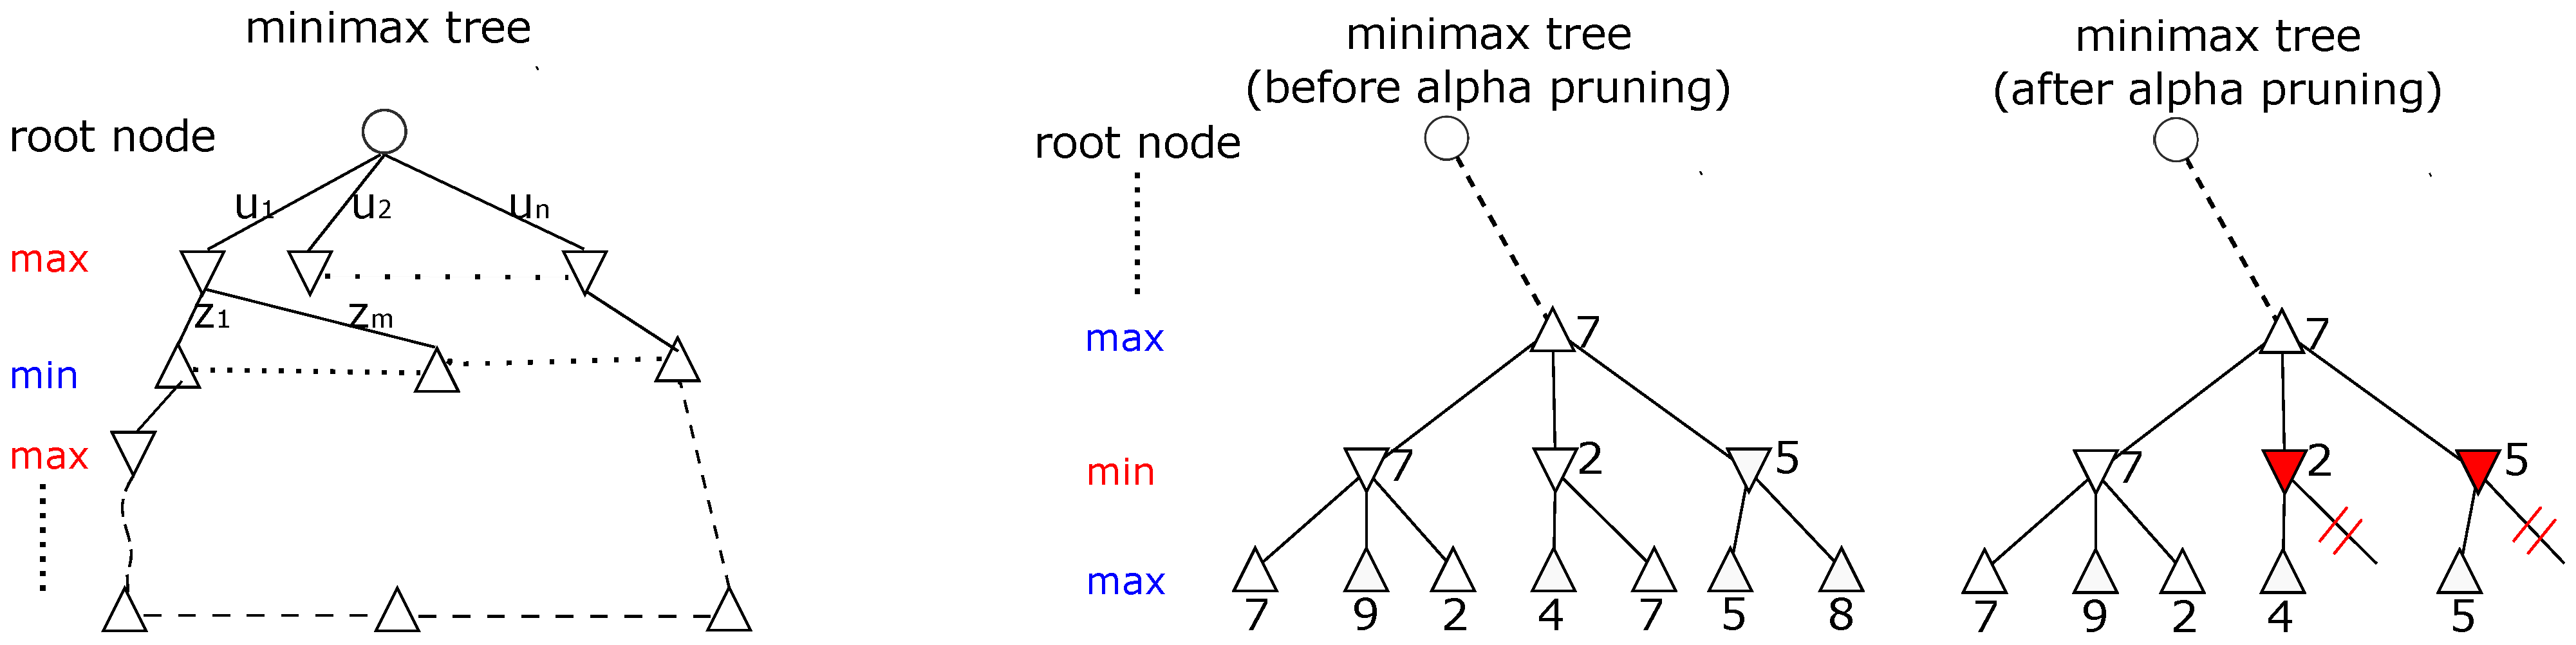
\includegraphics[height=3.5cm  ]{figs/MINMAX_tree.eps}
  \caption{A minimax tree with alpha pruning. $\bigtriangledown$  and $\bigtriangleup$  are nodes in which we compute the minimum or maximum value of its children. The value at the leaf nodes equals the $\mathrm{tr}(\Sigma_k) $. $\bigtriangledown$  and $\bigtriangleup$ nodes represent robot and target nodes, respectively. The filled $\bigtriangledown$ are pruned by alpha pruning.}
  \label{Minimaxtree1}
\end{figure*}

%\begin{algorithm}
%    \SetAlgoLined
%    $S_0\leftarrow\left\{(X_r(o), \Sigma_0)\right\}, \quad S_t\leftarrow\phi$ for $t=1,....,T$\\
%    $\mathcal{Z}=\left\{z_1,z_2,..., z_k\right\}$\\
%    $\mathbf{for} \quad\ t=1:T \quad\mathbf{do}$   \\
%      \quad $\mathbf{if}$ \quad NODE STATE ($\min$)\\
%         \qquad $\mathbf{for \quad all} \quad\ (X_r(t-1), \Sigma(t-1))\in S_{t-1}\quad\mathbf{do}$   \\
%         \qquad \qquad$\mathbf{for\quad all}\quad u_i\in \mathcal{U}$\\
%         \qquad \qquad \qquad $X_r(t)\leftarrow f(X_r(t-1),u_i)$\\
%        \qquad \qquad \qquad $S_t\leftarrow S_t \bigcup \left\{  (X_r(t), \Sigma(t-1))\right\}$
%        
%              \quad $\mathbf{else \quad if}$ \quad NODE STATE ($\max$)\\
%         \qquad $\mathbf{for \quad all} \quad\ (X_r(t), \Sigma(t-1))\in S_{t}\quad\mathbf{do}$   \\
%         \qquad \qquad$\mathbf{for\quad all}\quad z_i\in \mathcal{Z}$\\
%         \qquad \qquad \qquad $\Sigma(t) \leftarrow \rho (X_r(t), z_i, \Sigma(t-1))$\\
%        \qquad \qquad \qquad $S_t\leftarrow S_t \bigcup \left\{  (X_r(t), \Sigma(t))\right\}$\\
%
%          $\mathbf{for} \qquad t=1:T$  do\\
%        
%       \quad $\mathbf{if}$ TERMINAL-TEST (Max) \\
%        \qquad for each $S_t$ do\\
%        \qquad  \qquad$\mathcal{V} \leftarrow (max\Tr(\Sigma_i(t)), S_t(i))$\\
%        \qquad  \qquad$t \leftarrow t-1 $ \\
%        
%         \quad       $\mathbf{if}$ TERMINAL-TEST (Min) \\
%        \qquad for each $S_t$ do\\
%        \qquad  \qquad$\mathcal{V} \leftarrow (minimax\Tr(\Sigma_i(t)), S_t(i))$\\
%        \qquad  \qquad$t \leftarrow t-1 $ \\
%        
%       $\mathbf{return} \quad\mathcal{V}$
%    \caption{The minimax algorithm}
%    \label{minimax} 
%\end{algorithm}

\subsection{Alpha-Beta Pruning}
As a first step in reducing the size of the tree, we use alpha-beta pruning~\cite{russell2009artificial}. The main idea in alpha-beta  pruning is that if we have explored a part of the tree, we have an upper or lower bound on the optimal minimax value. For example, in alpha pruning where consider the upper bound, when exploring a new node, $n_i$, if we find that the minimax value of the subtree rooted at $n_i$ is greater than the upper bound found, that subtree does not need to be explored further. This is because an optimal strategy will never prefer a strategy that passes through $n_i$ since there exists a better control policy in another part of the tree. Note that $n_i$ must be a robot node. Figure~\ref{Minimaxtree1} shows an example of alpha-beta pruning. Target nodes cannot be pruned since the robot has no control over the actual measurement values. That is, we only apply alpha-pruning. When the measurements and target's motion is known to be adversarial, then full alpha-beta pruning can be applied. In such a case, the target nodes can be pruned away as well.

%\begin{algorithm}[h]
%   \SetAlgoLined
%   $\mathbf{function} $ alpha(Node,alpha,beta,MinimaxState)\\
%   \qquad  $\mathbf{if}$ Node.Deep == End \\
%    \qquad \qquad $X_r(t)\leftarrow f(X_r(t-1),u_i)$\\
%    \qquad \qquad $S_t\leftarrow S_t \bigcup \left\{  (X_r(t), \Sigma(t-1))\right\}$\\    
%    \qquad \qquad BestValue = Node.trace(Covariance);\\
%    \qquad  $\mathbf{esle\quad if}$ MinimaxState == Max\\
%      \qquad \qquad BestValue = alpha;\\
%    \qquad \qquad  //Recurse for all children of node. \\
%    \qquad \qquad $\mathbf{for}$ i=1:Node.children.length\\
%        \qquad  \qquad \quad $X_r(t)\leftarrow f(X_r(t-1),u_i)$\\
%    \qquad \qquad \quad $S_t\leftarrow S_t \bigcup \left\{  (X_r(t), \Sigma(t-1))\right\}$\\
%      \qquad \qquad \quad  ChildValue = alpha(child,alpha,beta,Min)\\
%      \qquad  \qquad \quad Bestvalue = $\max$(Bestvalue,ChildValue)\\
%     \qquad  \qquad \quad $\mathbf{if}$ (beta $<=$ BestValue) \\
%          \qquad  \qquad \qquad      break;//Do the alpha pruning\\
%          \qquad         $\mathbf{return} $ \quad Bestvalue\\
%      \qquad   $\mathbf{else}$ \\
%        \qquad \qquad BestValue = alpha;\\
%    \qquad \qquad  //Recurse for all children of node. \\
%    \qquad \qquad $\mathbf{for}$ i=1:Node.children.length\\
% \qquad \qquad \quad $\Sigma(t) \leftarrow \rho (X_r(t), z_i, \Sigma(t-1))$\\
%       \qquad \qquad \quad $S_t\leftarrow S_t \bigcup \left\{  (X_r(t), \Sigma(t))\right\}$\\
%      \qquad \qquad \quad  ChildValue = alpha(child,alpha,beta,Max)\\
%      \qquad  \qquad \quad Bestvalue = $\min$(Bestvalue,ChildValue)\\
%     \qquad  \qquad \quad $\mathbf{if}$ (beta $<=$ BestValue) \\
%          \qquad  \qquad \qquad      break;//Do the beta pruning\\
%   \qquad         $\mathbf{return} $ \quad Bestvalue\\
%
%   $S_0\leftarrow\left\{(X_r(0), X_o(0),\Sigma_0)\right\}$ \\
%   $\mathcal{Z}=\left\{z_1,z_2,..., z_k\right\}$\\                  
%       \qquad $\mathcal{V} \leftarrow $alpha(StartNode,$-\infty$,$\infty$,Min)\\
%       $\mathbf{return} \quad\mathcal{V}$
%       
%   \caption{The minimax  pruning algorithm}
%   \label{minimax_pruning} 
%    
%\end{algorithm}


\subsection{Algebraic Redundancy Pruning}    

%Our main contribution is to provide an algorithm with
%complexity lower than that of Alpha Pruning and performance better
%than that of the greedy policy. 

Vitus et al.~\cite{vitus2012efficient} presented algebraic redundancy pruning of search trees (not minimax trees) for linear systems with state-independent noise. The key idea is that  if a node, $n_i$, has higher uncertainty than another node, $n_j$ at the same level, then any descendant of $n_i$ will always have higher uncertainty than some descendant of $n_j$. Therefore, $n_i$ is redundant and can be pruned away. They use the monotonicity and concavity of the Riccati mapping in linear systems with state-independent noise to prove the following result. 

\begin{theorem}[Algebraic Redundancy~\cite{vitus2012efficient}]
Let $\mathcal{H} = \{(X^j_r(t),\Sigma^j_t)\}$ be a set of $n$ nodes at the same level of the tree. If there exist non-negative constants $\alpha_1, \alpha_2, \dots, \alpha_k$ such that,
$$   \Sigma^p_t\succeq \sum^k_{i=1}{\alpha_j\Sigma^j_t}\quad \text{and} \quad \sum^k_{i=1}{\alpha_i} = 1$$
then the node $\left(X^p_r(t),\Sigma^p_t\right)$ is regarded as algebraically redundant\footnote{$M \succeq  N$ represents that $M-N$ is positive semi-definite.} with respect to $\mathcal{H}\setminus\{(X^p_r(t),\Sigma^p_t)\}$ and $(X^p_r(t),\Sigma^p_t)$ and all of its descendants can be pruned without eliminating the optimal solution from the tree.
\label{thm:fromvitus}
\end{theorem}

They prove that the trace of any successor of $(X^p_r(t),\Sigma^p(t))$ cannot be lower than one of the successors of $\mathcal{H}\setminus\{(X^p_r(t),\Sigma^p(t))\}$. Our main insight is that a similar redundancy constrained can be defined for the non-linear case with suitable additional constraints as described below.

We extend these ideas for minimax trees with possibly state-dependent noise. We first prove the monotonicity of state-dependent Riccati equation.
\begin{lemma}
Let $A$ and $B$ be two nodes in the same level of the minimax tree. If
$H\Sigma_{t}^AH^T+S^A \succeq H\Sigma_{t}^BH^T+ S^B$
 then after applying one step of the Riccati equation, we have $\rho(\Sigma_{t}^A)\succeq \rho(\Sigma_{t}^B)$. 
 \label{lemma:mono}
\end{lemma}
We will show conditions under which a node $A$ is redundant with respect to a set of nodes, termed as candidate set, that is already present in the tree. Figure~\ref{fig:candidate set} shows an example.
\begin{definition} 
Let $\mathcal{H}$ be a set of nodes. The set $\mathcal{H}$ is called as a \emph{candidate set} with respect to some node $A$ if (i) the nodes in $\mathcal{H}$ are at the same level as that of $A$; and (ii) every node $B\in\mathcal{H}$ is on the optimal minimax path for the subtree rooted at the least common ancestor of $A$ and $B$.
\end{definition}

\begin{figure}[h] 
  \centering
  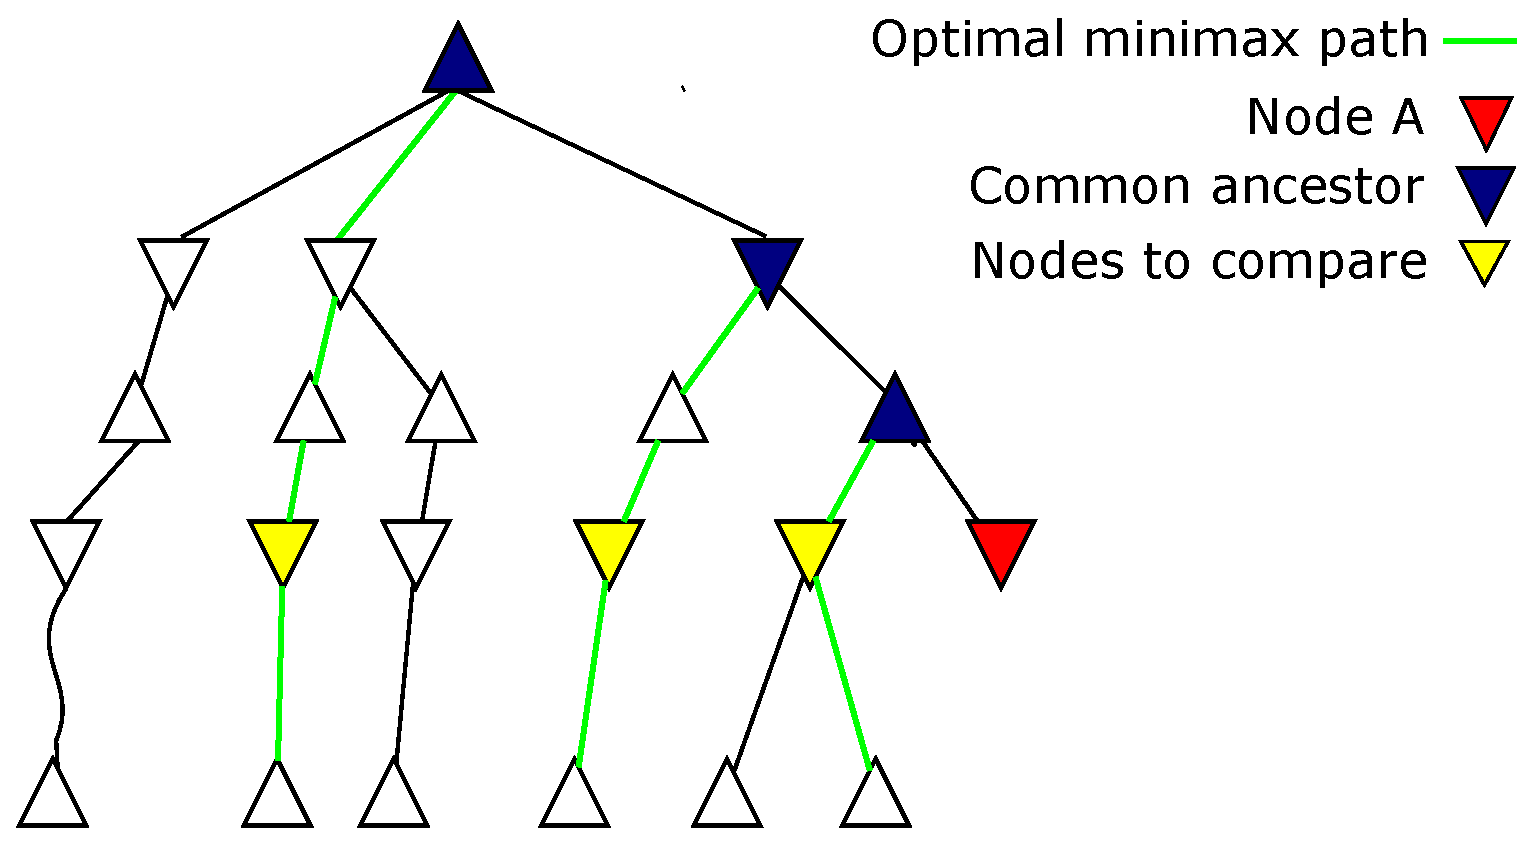
\includegraphics[height=3.5cm  ]{figs/minimax_pruning.eps}
  \caption{Nodes in the candidate set, $\mathcal{H} = \{(X^i_r(t),\hat{X}^i_o(t),\hat{\Sigma}^i_t)\}$, of node $A$ are marked in yellow. Their least common ancestor is marked with in.}
  \label{fig:candidate set}
\end{figure}

Before we present the full details, we list the conditions that will be used in Theorem~\ref{thm:main}. We have more conditions since pruning with state-dependent noise is a general version of Theorem~\ref{thm:fromvitus}. 

Let $\mathcal{H} = \{(X^i_r(t),\hat{X}^i_o(t),\hat{\Sigma}^i_t)\}$ be the candidate set of $N$ nodes with respect to some node $A=(X^A_r(t),\hat{X}^A_o(t),\hat{\Sigma}^A_t)$. The conditions are as follows:
\begin{enumerate}[label=(C\arabic*)]
\item the robot and estimated target states are identical, \ie{}  $X^A_r(t)=X^i_r(t)$ and $\hat{X}^A_o(t)=\hat{X}^i_o(t)$ for all $i$ in $\mathcal{H}$;\footnote{For time-invariant linear systems with constant $H$ and $C$, condition (C1) is not required since all the covariance matrices are updated through the same Kalman filter Riccati equations.}
\item the least common ancestor of $A$ with any other node in $\mathcal{H}$ is a min (robot) node;
\item the least common ancestor of $A$ with any other node in $\mathcal{H}$ is a max (target) node;
\item there exist non-negative $\alpha_i$ such that for any positive integer $M$:
%\end{enumerate}
\begin{equation}\label{c1}
  H_t\Sigma_t^AH_t^T \succeq   \sum^{N}_{i=1}\alpha_i \left( H_t\Sigma_t^iH_t^T + MaI_{2\times 2}\right)
\end{equation}
%\begin{enumerate}[label=(\roman*)]
 %\setcounter{enumi}{5}
\item there exist non-negative $\alpha_i$ such that for any positive integer $M$:
%\end{enumerate}
\begin{equation}\label{c2}
  H_t\Sigma_t^AH_t^T \preceq   \sum^{N}_{i=1}\alpha_i \left( H_t\Sigma_t^iH_t^T + MaI_{2\times 2}\right)
\end{equation}
where in Equations~\ref{c1} and \ref{c2}, we have $a=\left(\delta_1^2 +\delta_2^2\mathcal{C}\right)$ and $\sum^{N}_{i=1}\alpha_i =1$.
\end{enumerate}


%\begin{figure}[h] \label{Minimaxtree}
%  \centering
%  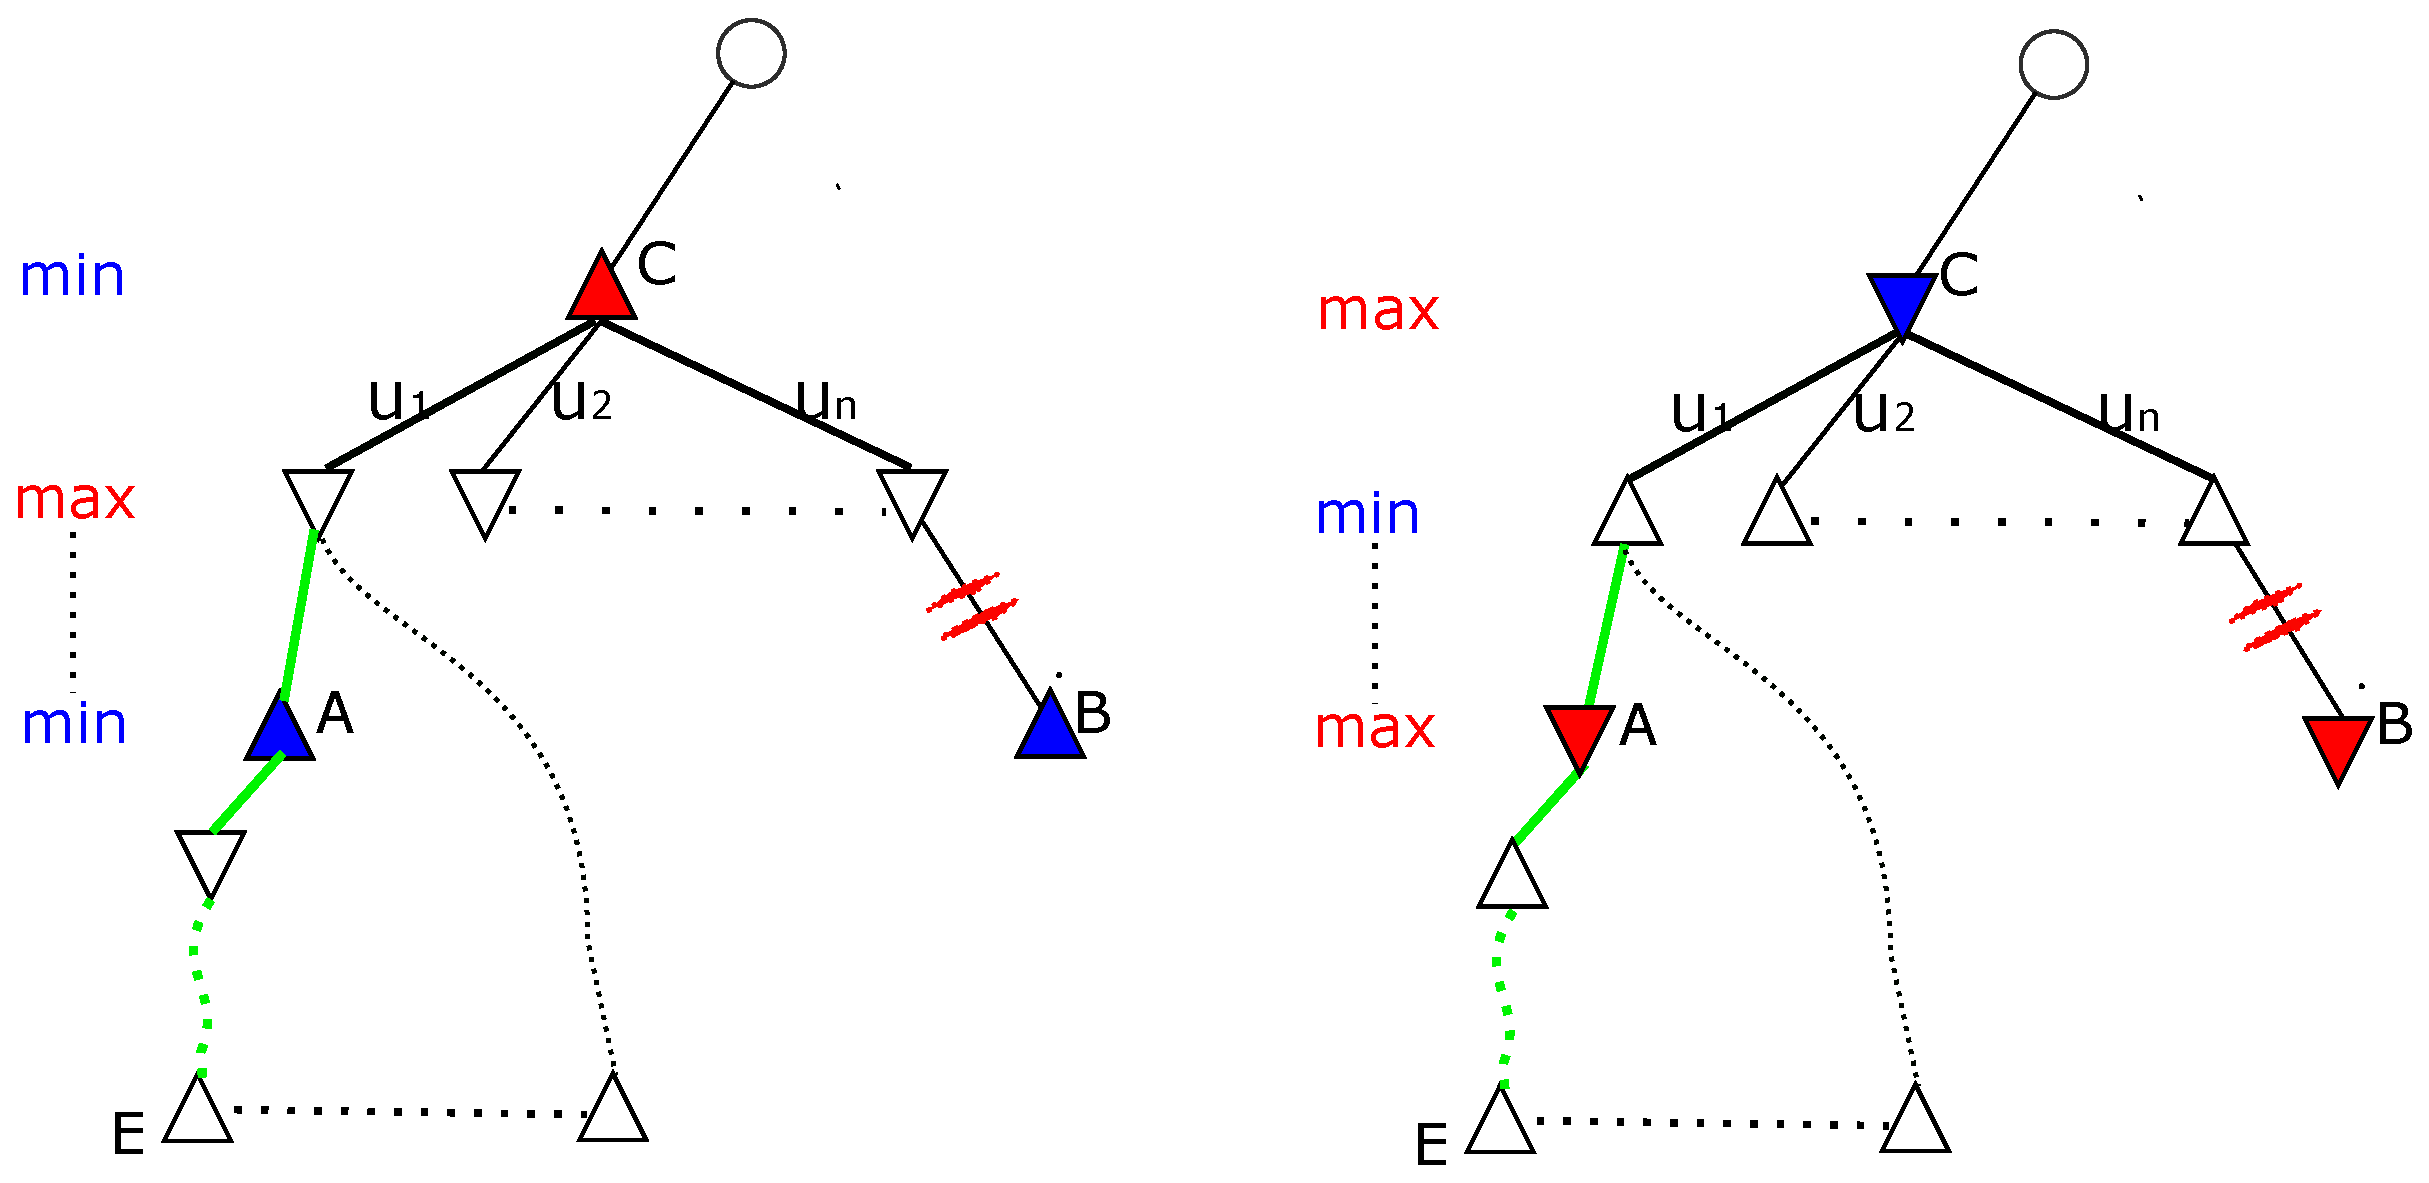
\includegraphics[height=3.5cm  ]{figs/ARpruning.eps}
%  \caption{State-dependent Linear Algebraic Redundancy Pruning}
%  \label{Minimaxtree}
%\end{figure}
   
Our main result is stated as follows.   
\begin{theorem}\label{StateDependentAR}[State-dependent Algebraic Redundancy]
Let $\mathcal{H} = \{(X^i_r(t),\hat{X}^i_o(t),\hat{\Sigma}^i_t)\}$ be the candidate set of $N$ nodes with respect to some node $A=(X^A_r(t),\hat{X}^A_o(t),\hat{\Sigma}^A_t)$. If the node $A$ satisfies (C1), (C2) and (C4), then there exists a node in $\mathcal{H}$, say $B$, such that:
\begin{equation*}
\text{tr}(\Sigma^A_{t+M}) \ge \text{tr}(\Sigma^B_{t+M}).
\end{equation*}

Similarly, if node $A=(X^A_r(t),\hat{X}^A_o(t),\hat{\Sigma}^A_t)$ satisfies (C1),  (C3) and (C5), then there exists a node in $\mathcal{H}$, say $B$, such that:
\begin{equation*}
\text{tr}(\Sigma^A_{t+M}) \le \text{tr}(\Sigma^B_{t+M}).
\end{equation*}
In both cases, the node $A$ can be pruned from the minimax tree without affecting the optimal policy.
\label{thm:main}
\end{theorem}

We use the above result to prune away nodes while building the tree. Note that the algebraic redundancy pruning is more effective when the tree is being built in a breadth-first fashion (since we compare nodes at the same level). On the other hand, the alpha-beta pruning is useful only when the tree is built in a depth-first fashion. In order to apply both pruning strategies, the tree must be built depth-first. While adding a new node to the tree, we check whether the conditions in Theorem~\ref{thm:main} are satisfied with respect to all other existing nodes at the same level. In order to check for the optimal path, we require at least one path to a leaf node from the current node. Therefore, the conditions can be checked for all predecessors of the current node under consideration. If the conditions are met for any predecessor, then the predecessor node (and all its descendants) are pruned from the tree. 

Since $\mathcal{H}$ can be of any size, checking for conditions (C4) and (C5) can be computationally expensive (require solving a Linear Matrix Inequality). Instead, we can restrict $\mathcal{H}$ to contain only one node. This will result in sub-optimal pruning but will save computational time. In the next section, we describe more ways of saving computational time at the expense of optimality.

\subsection{Sub-optimal Pruning algorithm}  
We can further reduce the number of branches at the expense of losing optimality by relaxing the alpha-pruning and algebraic redundancy constraints. We use two parameters $\epsilon_1 > 0$ and $\epsilon_2 > 0$ as relaxation parameters for alpha pruning and algebraic redundancy pruning, respectively. In each case, we bound the loss in optimality as a function of the parameters.

Specifically, while building the tree, we prune away a node if it satisfies either of the following two conditions.  When checking for alpha pruning, we prune a node if its alpha value is greater than or equal to the best minimax value found so far minus $\epsilon_1$. Similarly, we replace the constraint in Theorem~\ref{thm:main} with the following: 
\begin{equation}
  H_t(\Sigma_t^A+\epsilon_2)H_t^T \succeq  \sum^{N}_{i=1}\alpha_i \left[ H_t\Sigma_t^iH_t^T + M\left(\delta_1^2 +\delta_2^2\mathcal{C}\right)\right]
\end{equation}
By varying $\epsilon_1$ and $\epsilon_2$, we can vary the number of nodes in the search tree. Next we bound the resulting loss in the optimality of the algorithm.

\begin{theorem}[$\epsilon_1$-alpha pruning]
Let $J_{2k}^\ast=\Tr(\hat{\Sigma}_{2k}^\ast)$ be the optimal minimax value returned by the full enumeration tree. If $J_{2k}^{\epsilon_1}=\Tr(\hat{\Sigma}_{2k}^{\epsilon_1})$ is the value returned by the $\epsilon_1$--alpha pruning algorithm, then
$0\leq J_{2k}^{\epsilon_1}-J_{2k}^\ast\leq\epsilon_1.$
\end{theorem} 

The proof follows directly from the fact that if a node on the optimal policy, say $n_i$ is pruned away, then the alpha value at $n_i$ is at most the alpha value of some other node, say $n_j$, that is present in the tree minus $\epsilon_1$. The alpha value of $n_j$ cannot be less than the value returned by the $\epsilon_1$ algorithm. The bound for $\epsilon_2$-algebraic redundancy pruning is more complicated.

\begin{theorem}
[$\epsilon_2$-State dependent algebraic redundancy pruning]
Let $J_{2k}^\ast=\Tr(\hat{\Sigma}_{2k}^\ast)$ be the optimal minimax value returned by the full enumeration tree of $2k$ levels. If $J_{2k}^{\epsilon_2}=\Tr(\hat{\Sigma}_{2k}^{\epsilon_2})$ is the value returned by the $\epsilon_2$--algebraic redundancy pruning algorithm, then
$$
0\leq  J_{2k}^{\epsilon_2}-J_{2k}^\ast \leq B^{\epsilon_2}$$
where,
\begin{align*}
&B^{\epsilon_2} =\\
&\Tr\left\{  \sum^k_{j=0} \left[ \prod^j_{i=k-1}\left( F_i(\Sigma) \Phi_{2i}(\Sigma)\right)  \prod^{k-1}_{i=j}\left(  F_i(\Sigma) \Phi_{2i}(\Sigma)\right)^T \right]\epsilon_2 
 \right\}
 \end{align*}
where, $F_i(\Sigma)=C-CK_i(\Sigma)H_i$ and $K_i(\Sigma)$ is the Kalman gain given by $K_i(\Sigma)=\Sigma H_i^T(H_i\Sigma H^T_i+\Sigma_{w})^{-1}$, and $\Phi_{2k}(\cdot)$ is the application of the Riccati equation $\rho(\cdot)$, over $k$ measurement steps: 
$$\Phi_{2k}(\cdot) = \underbrace{\rho_{2(k-1)}(\rho_{2(k-2)}( \dots \rho_0(\cdot)))}_{\text{k  steps  }\rho(\cdot)}. $$
\label{thm:epsilon2bound}
\end{theorem}

By combining the two results, we get
$$0\leq  J_{2k}^{\epsilon_1,\epsilon_2}-J_{2k}^\ast \leq \max \left\lbrace \epsilon_1,B^{\epsilon_2} \right\rbrace.$$

\subsection{Online Execution of the Search Tree}  
\label{sec:online}

So far, we have discussed the problem of building the minimax tree. Once the tree is built, the robot can execute the optimal policy. At the root node, the robot executes the first control action along the optimal minimax path found. Then, the robot obtains a measurement. This measurement may not correspond to the worst-case measurement. Furthermore, the actual value of the measurement may not even be in the $k$ candidate measurements in the tree. Therefore, the updated target estimate may not correspond to a node in the tree. Instead, we compute find the node in the tree whose target estimate is closest to the actual one. We can use Bhattacharyya distance~\cite{bhattacharyya1943measure} to find the closest target estimate in the tree. The corresponding node then becomes the new root node of the tree. The optimal policy starting at that node is executed, iteratively. If the Bhattacharyya distance of the closest node is too large, we still can rebuild the whole minimax tree with the current target estimate as the root node. This process of executing the minimax tree online is shown in Figure~\ref{simulation_step}. 

\begin{figure}
  \centering
  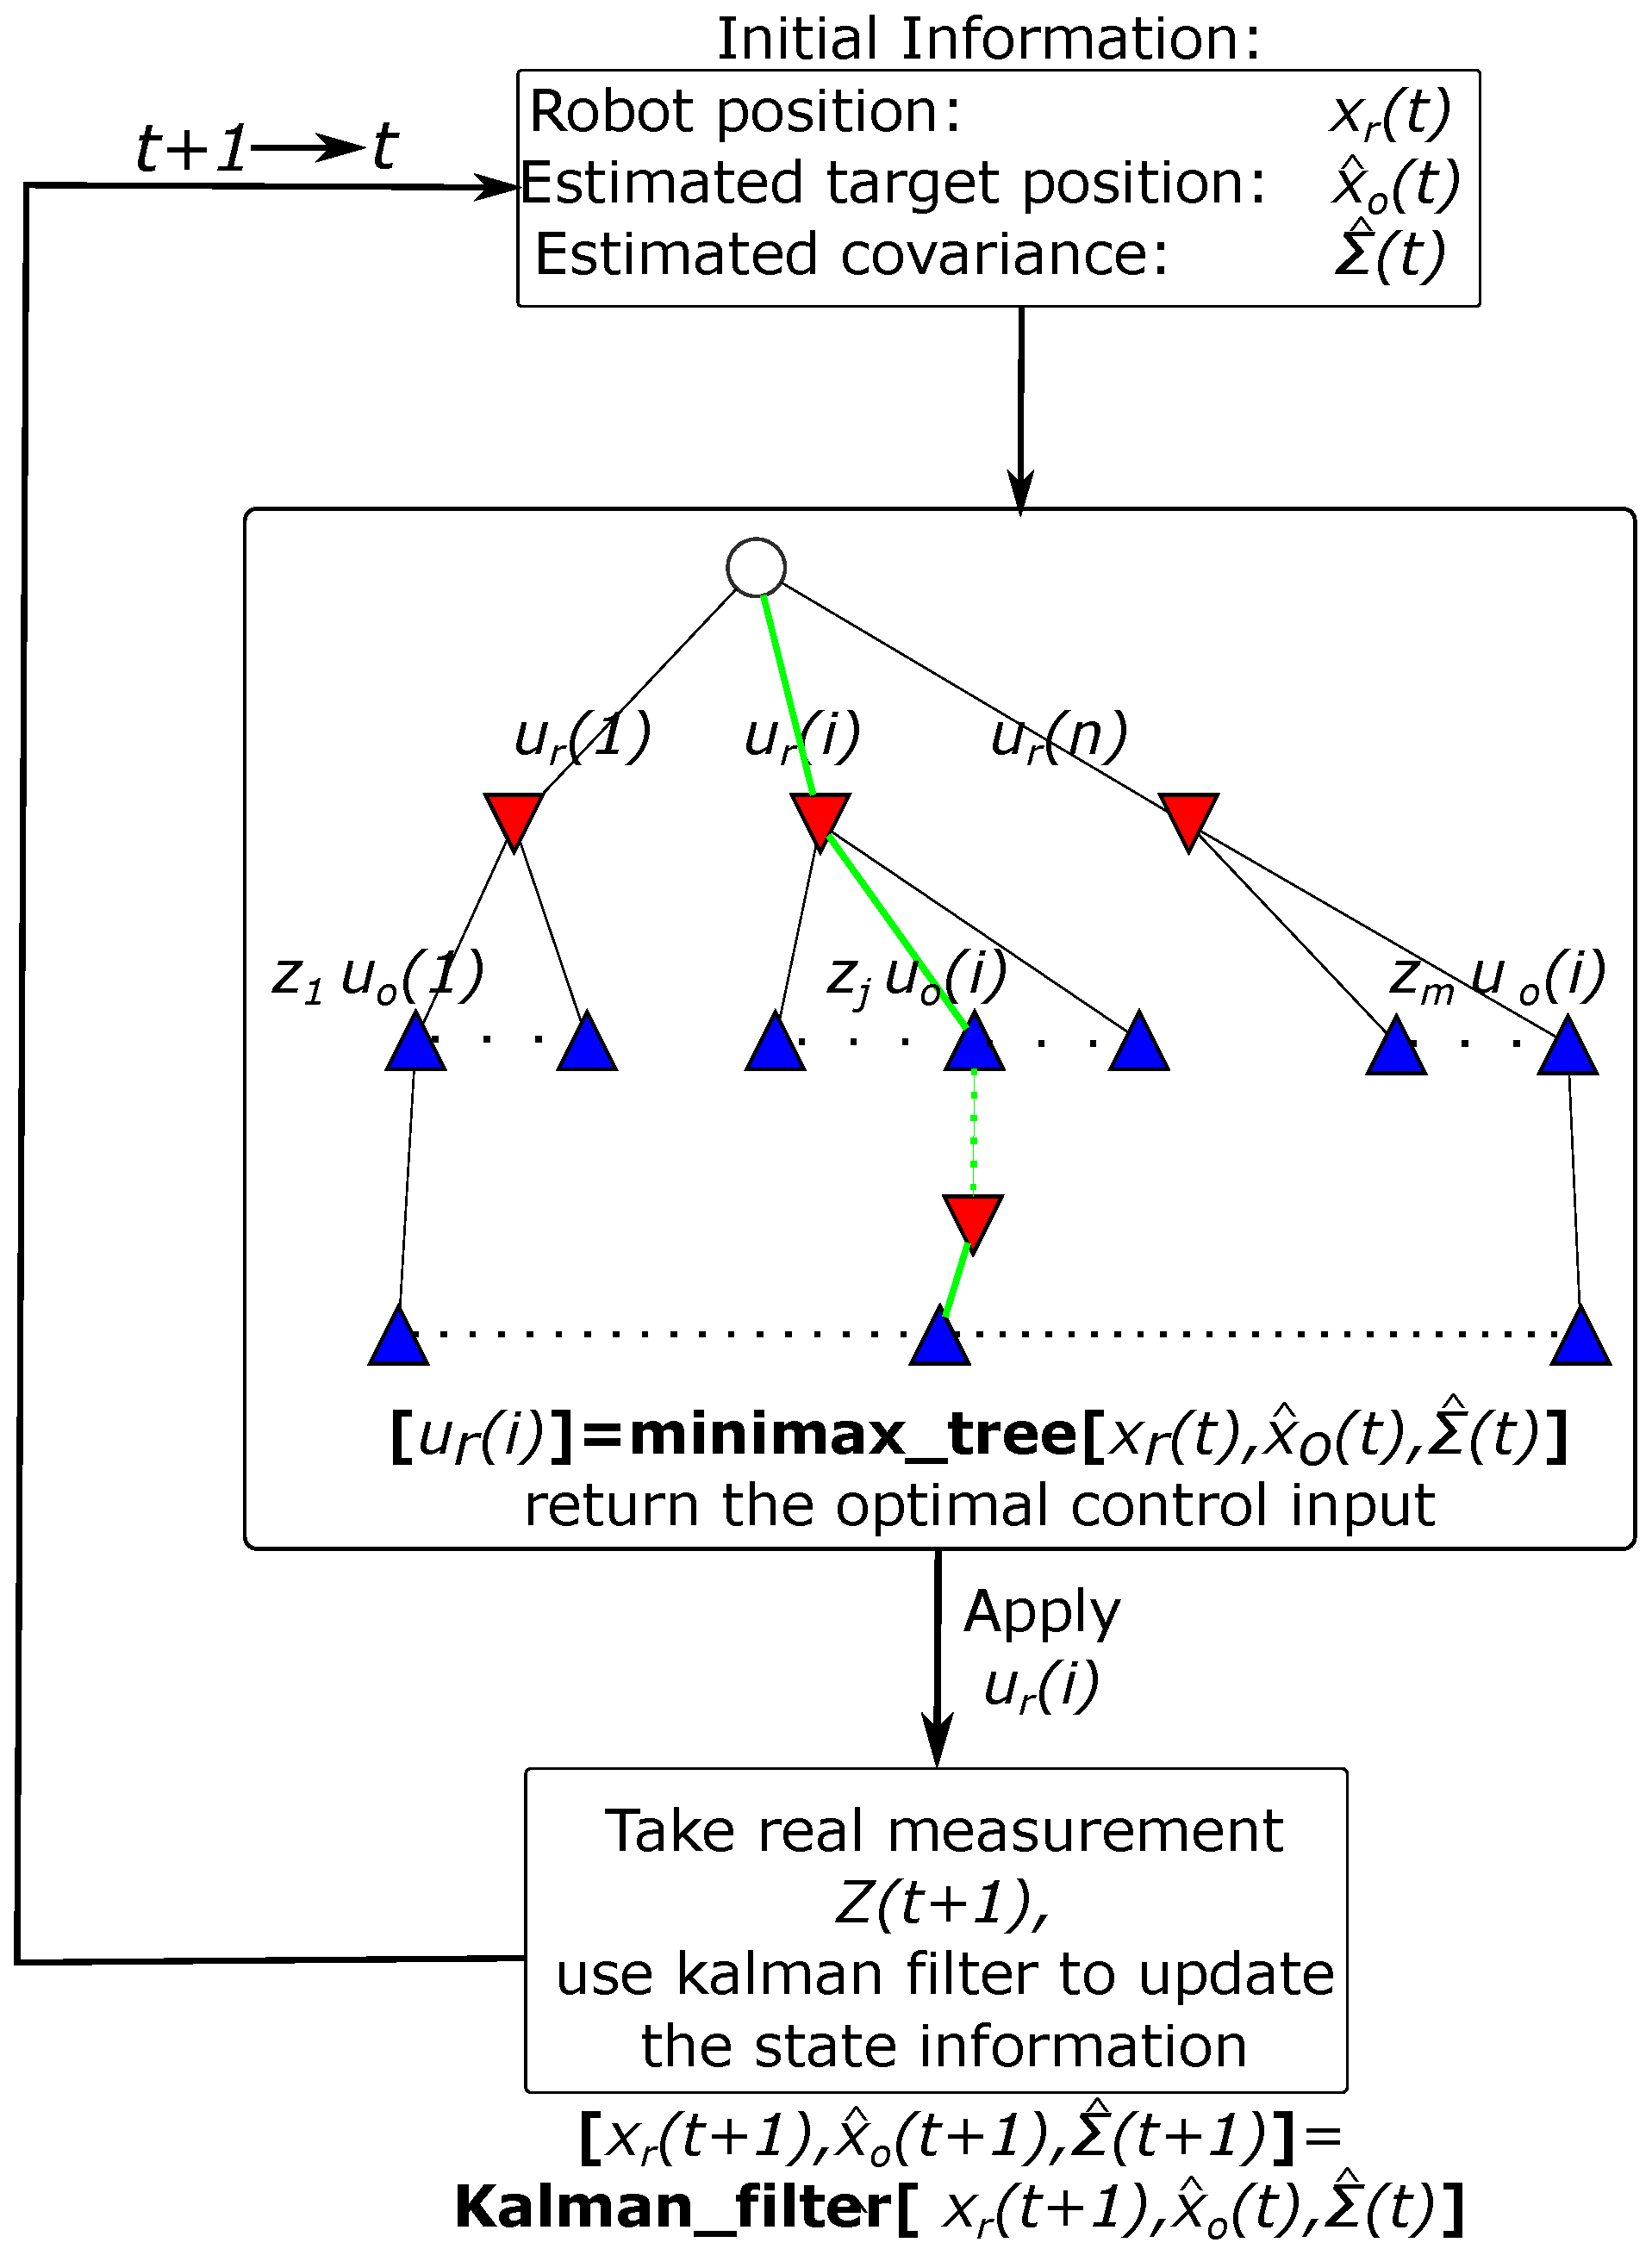
\includegraphics[height=7cm]{figs/simulation_step.eps}
  \caption{Online execution of the minimax tree. At each time step, the robot executes the first control action given by the tree and obtains a measurement of the target. If the measurement $Z(t+1)$ is close to one of the existing nodes, then that node is termed as the new root node. The tree can then extended to have a depth of $(k+1)$. If the new measurement $Z(t+1)$ is not close to any nodes, then the tree can be rebuilt with the current estimate as the root node.}
  \label{simulation_step}
\end{figure}





%%%%%%%%%%%%%%%%%%%%%%%%%%%%%%%%%%%%%%%%%%%%%%%%%%%%%%%%%%%%%%%%%%%%%%%%%%%%%%%%

\section{Simulations} \label{sec:sims}
We carry out three types of evaluations via simulations. First, we investigate the computational savings due to our algorithm by comparing the number of nodes in the pruned minimax tree and the full enumeration tree. Then, we study the effect of varying the $\epsilon_1$ and $\epsilon_2$ parameters on the number of nodes. Finally, we use the control policy given by our algorithm and execute it by drawing actual measurements from a random distribution. This represents a realistic scenario where the measurements are not necessarily adversarial. We demonstrate how our strategy can be used in such a case, and compare the average-case with the worst-case performance.

We start by describing the models used in the simulation. The robot follows a linear motion model and can choose from four actions at each time step:
 \begin{equation}
 \mathcal{U}_r=\left\{\begin{bmatrix}
    1.0    \\
   0   \\
\end{bmatrix}, \begin{bmatrix}
    0    \\
   1.0   \\
\end{bmatrix}, \begin{bmatrix}
    -1.0    \\
   0   \\
\end{bmatrix}, \begin{bmatrix}
   0    \\
   -1.0   \\
\end{bmatrix}\right\}
\label{eqn:simrobotmotionmodel}
\end{equation}

We build the tree using five candidate measurements at each step: $z(t)=\{z_1(t),z_2(t),\cdots, z_5(t) \}$. The five values are randomly generated by drawing from a Gaussian distribution.
 
\subsection{Comparing the Number of Nodes}

\begin{figure}[!htb]
  \centering
  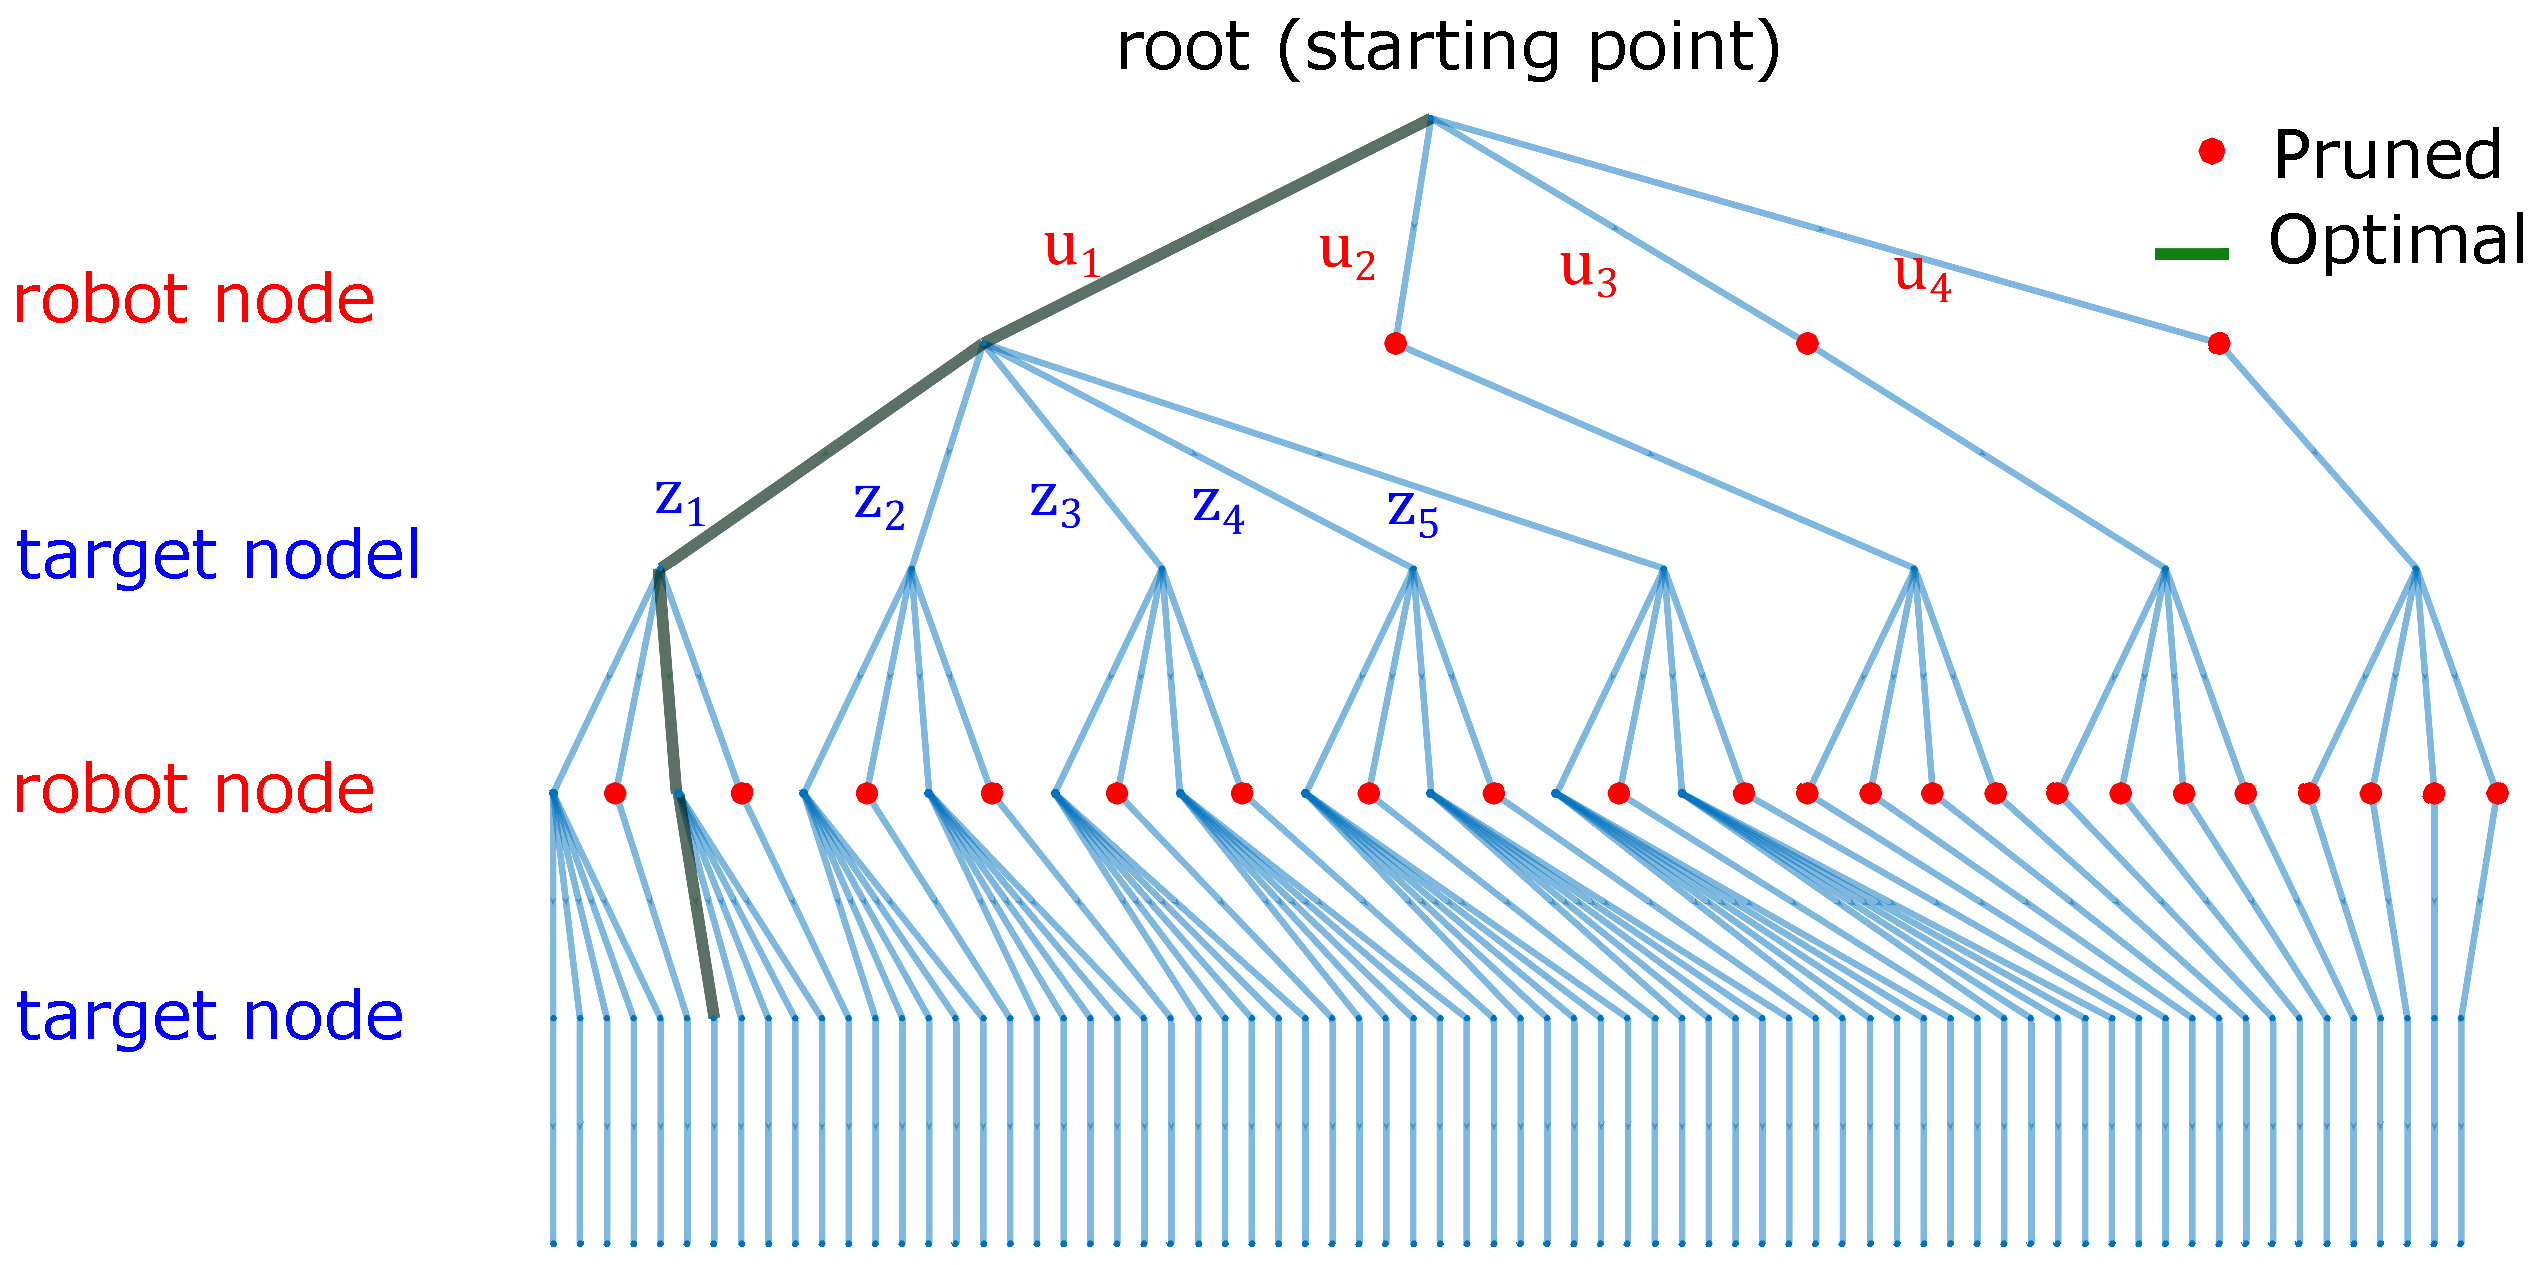
\includegraphics[width=8cm]{figs/Minimax5result.eps}
  \caption{A five-level minimax tree with pruning (189 nodes). Full enumeration has 505 nodes.}
  \label{Minimax5result}
\end{figure}

Figure~\ref{Minimax5result} shows an example of a five-level minimax tree with pruning. Figure~\ref{Number_of_nodes_Time_step3} shows the number of nodes  in the minimax tree after pruning and the number of nodes in a full enumeration tree, respectively. We prune a node by comparing it to the nodes already explored. More nodes will be pruned if initial nodes encountered are ``close'' to the optimal policy. For instance, if the first set of nodes explored happen to be  the optimal control law that drives the robot close to the target, then we expect the nodes encountered later will be pruned earlier in the process. To provide a fair assessment, we generate the search trees for various true positions of the target. Figure~\ref{Number_of_nodes_Time_step3} shows the average and standard deviation of the number of nodes.

Figure~\ref{Number_of_nodes_Time_step3} shows that our algorithm prunes orders of magnitudes of nodes from the full enumeration tree. For a tree with depth 13, there are $8.08\times 10^7$ nodes in the full tree  but the same optimal solution can be computed using $4.36\times 10^5$ nodes with our pruning strategy.

%The effectiveness of alpha-beta pruning and algebraic redundancy pruning are highly depended on the order in which the states are examined. If a good node had been generate first, we would have been able to prune more nodes. If this can be done, for a $m$ level tree, it turns out that alpha-beta needs examine only $O(b^{m/2})$ nodes to pick the best move \cite{russell2009artificial}. With our algebraic redundancy pruning, better results can be achieved. 

By sacrificing optimality, we can prune even more nodes. We evaluate this by varying $\epsilon_1$ and $\epsilon_2$ individually first, and then jointly. As shown in Figure~\ref{Number_of_nodes_with_pruning},  $\epsilon_1$-alpha pruning is relatively better at reducing the size of the minimax tree. This is intuitive because $\epsilon_1$-alpha pruning condition compares  nearly every pair of nodes at the same depth. $\epsilon_2$-algebraic redundancy pruning, on the other hand, requires more conditions to be satisfied. Nevertheless, Figure~\ref{Number_of_nodes_with_pruning} shows that by sacrificing optimality, the number of nodes can be substantially reduced.

\begin{figure}[!htb]
  \centering
  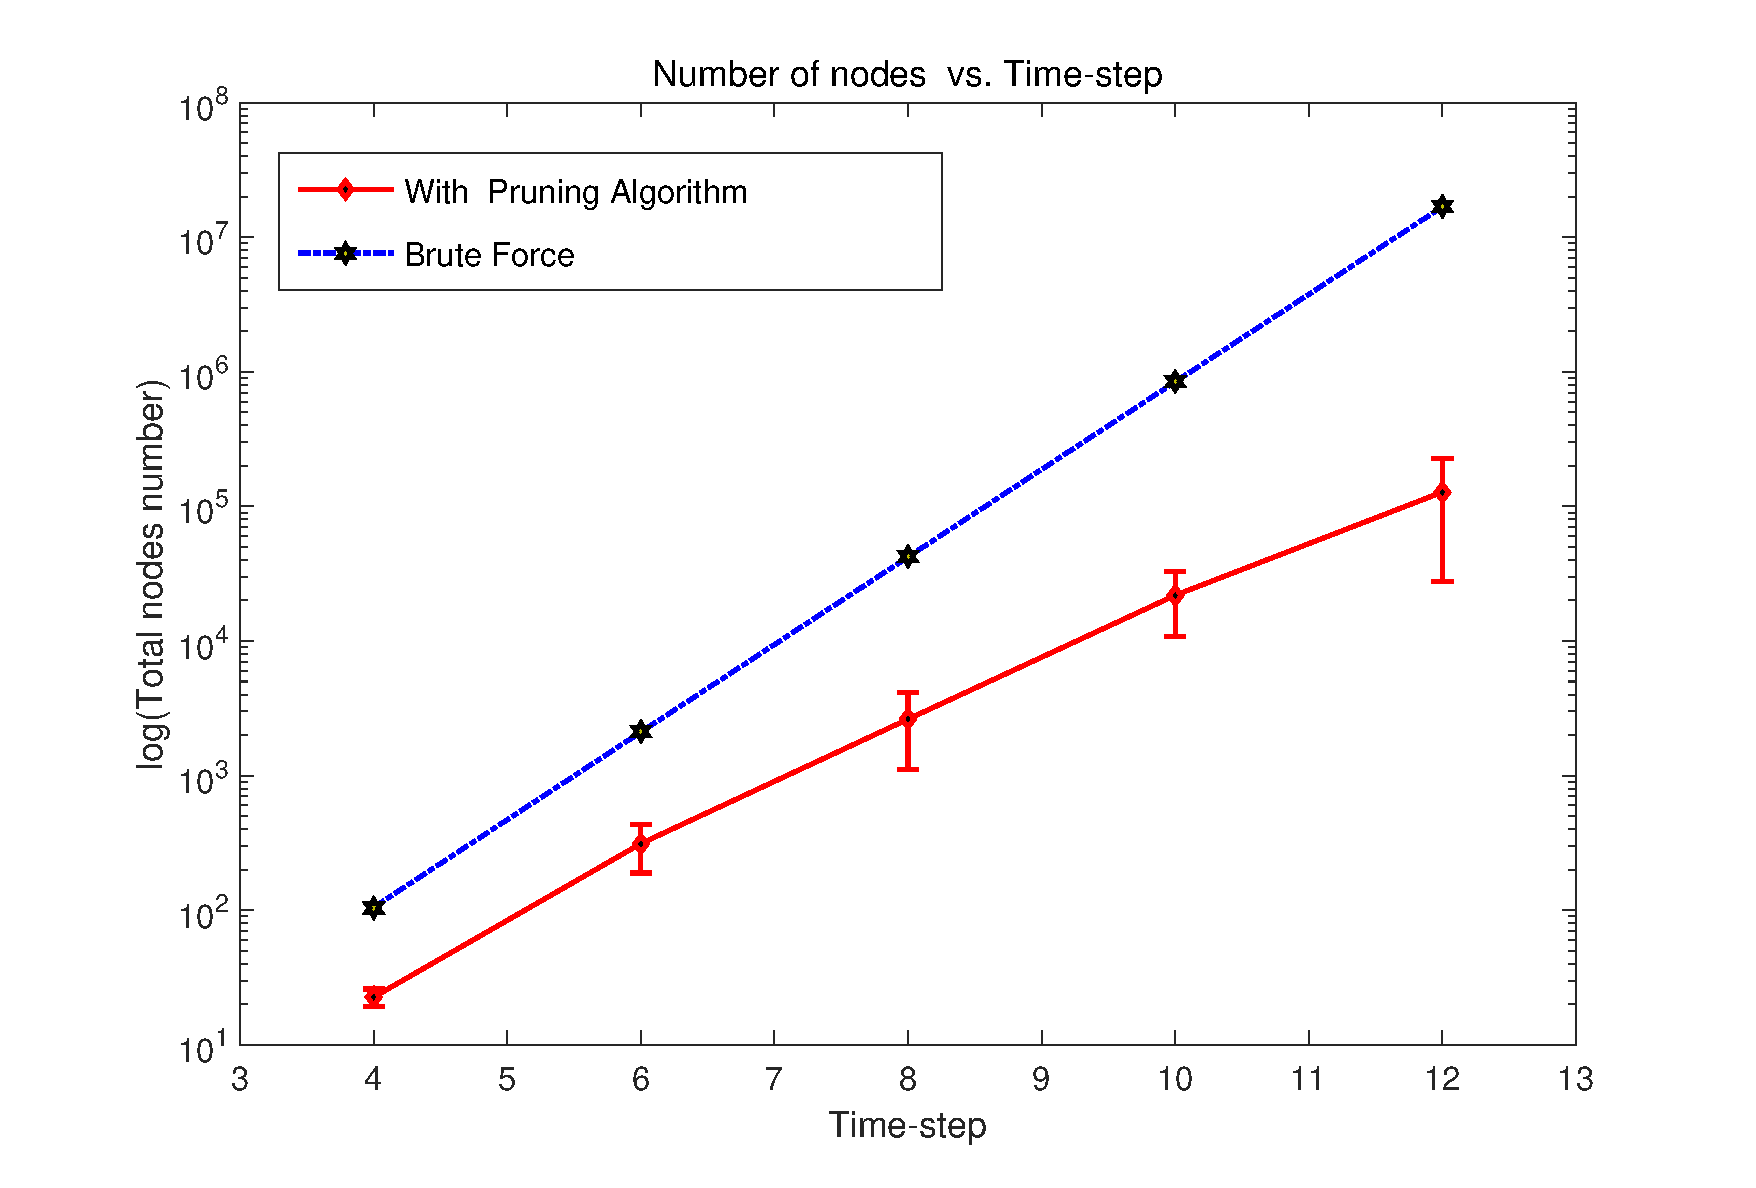
\includegraphics[width=8cm]{figs/Number_of_nodes_Time_step3.eps}
  \caption{Comparison of the number of total nodes generated for minimax tree. Note that the $y$ axis is $\log$ scale.}
  \label{Number_of_nodes_Time_step3}
\end{figure}

\begin{figure}[!htb]
  \centering
  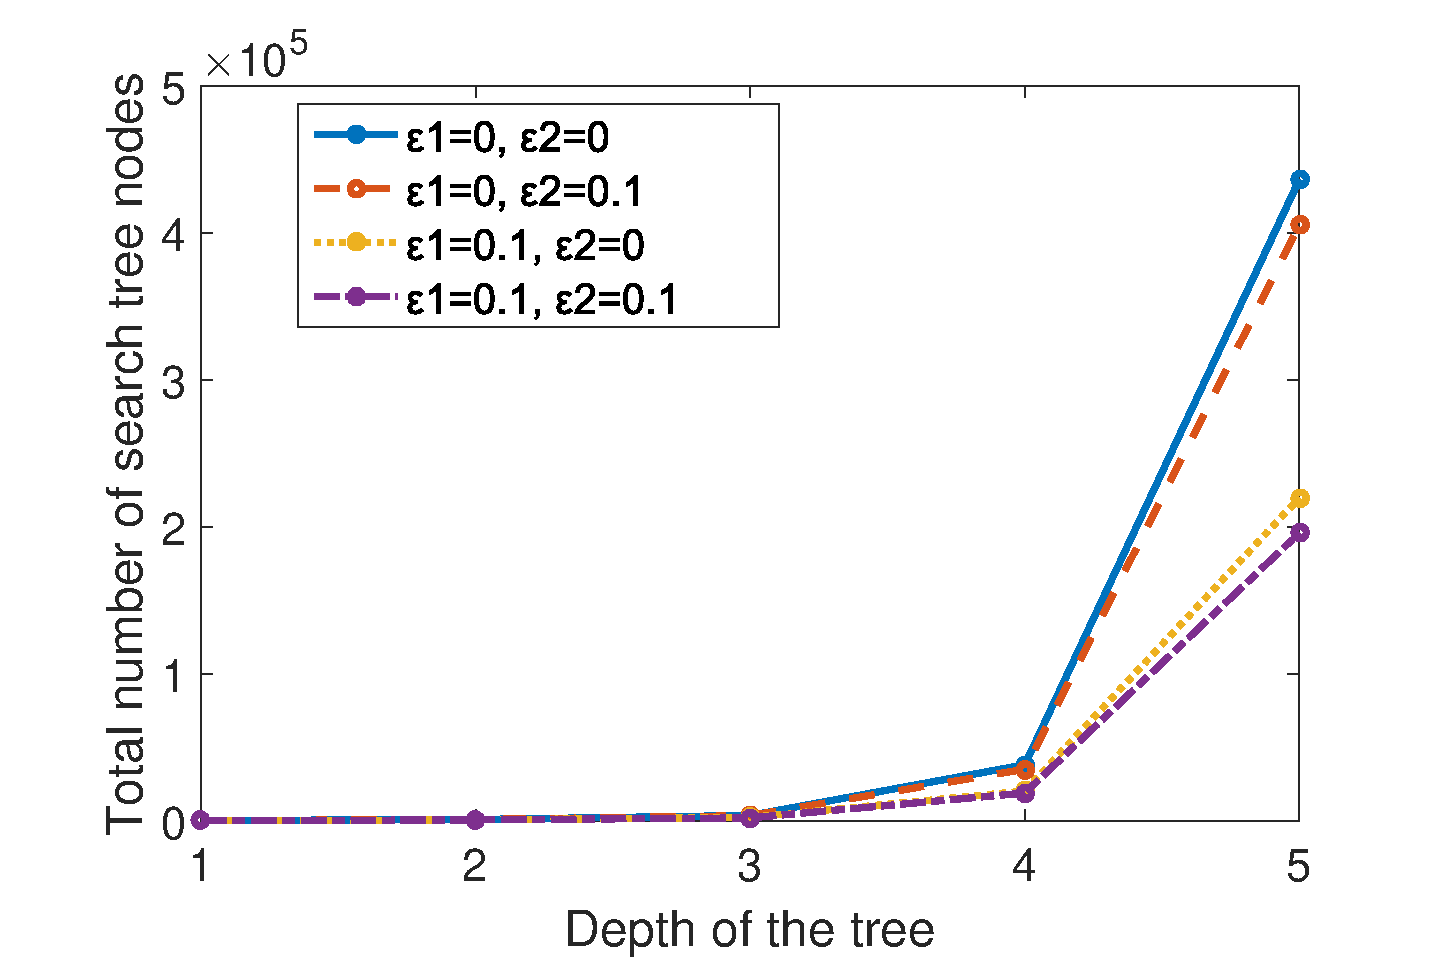
\includegraphics[width=8cm]{figs/Number_of_nodes_with_pruning.eps}
  \caption{Effect of the $\epsilon_1$ and $\epsilon_2$ relaxation parameters on the number of nodes in the search tree. The baseline case is the optimal solution with alpha pruning and algebraic redundancy with both parameters set to zero.}
  \label{Number_of_nodes_with_pruning}
\end{figure}
  

\subsection{Gazebo Simulations}

We used the Gazebo simulation environment~\cite{koenig2004design} to evaluate the online execution of the minimax tree policy given in Section~\ref{sec:online}. Figure~\ref{Gazebo} shows the setup. The tracking robot and the target are simulated using the model of a differential-drive robot (Pioneer 3DX). The motion model for the robot is the same as that reported in the previous section (Equation~\ref{eqn:simrobotmotionmodel}). For simulations where the target is mobile, the motion model and possible control laws are given by:
 $$ X_o(t+1)=X_o(t)+u_o(t)+v(t)$$

\begin{equation}
\mathcal{U}_o= \left\{\begin{bmatrix}
    0.6    \\
   0   \\
\end{bmatrix}, \begin{bmatrix}
    0    \\
   0.6   \\
\end{bmatrix}, \begin{bmatrix}
    -0.6    \\
   0   \\
\end{bmatrix}, \begin{bmatrix}
    0    \\
   -0.6   \\
\end{bmatrix}, \begin{bmatrix}
    0    \\
   0   \\
\end{bmatrix}\right\}
\label{eqn:simtargetmotionmodel}
\end{equation}

We simulate the following three scenarios:
\begin{enumerate}
\item The robot tracks a stationary target. The simulated measurements are the worst-case ones. Figure~\ref{online1} shows the robot's trajectory, the simulated measurements, and the estimation results.
\item The robot tracks a target which moves with a randomly drawn control inputs from the four options given in Equation~\ref{eqn:simtargetmotionmodel}. The simulated measurements are the worst-case ones. Figure~\ref{online2} shows the results from this simulation.
\item The robot tracks a target that actively chooses adversarial control inputs to ``escape'' from the robot. Specifically, the target chooses actions that will maximize the estimation uncertainty. Figure~\ref{case3} shows the simulation results.
\end{enumerate}


\begin{figure}
  \centering
  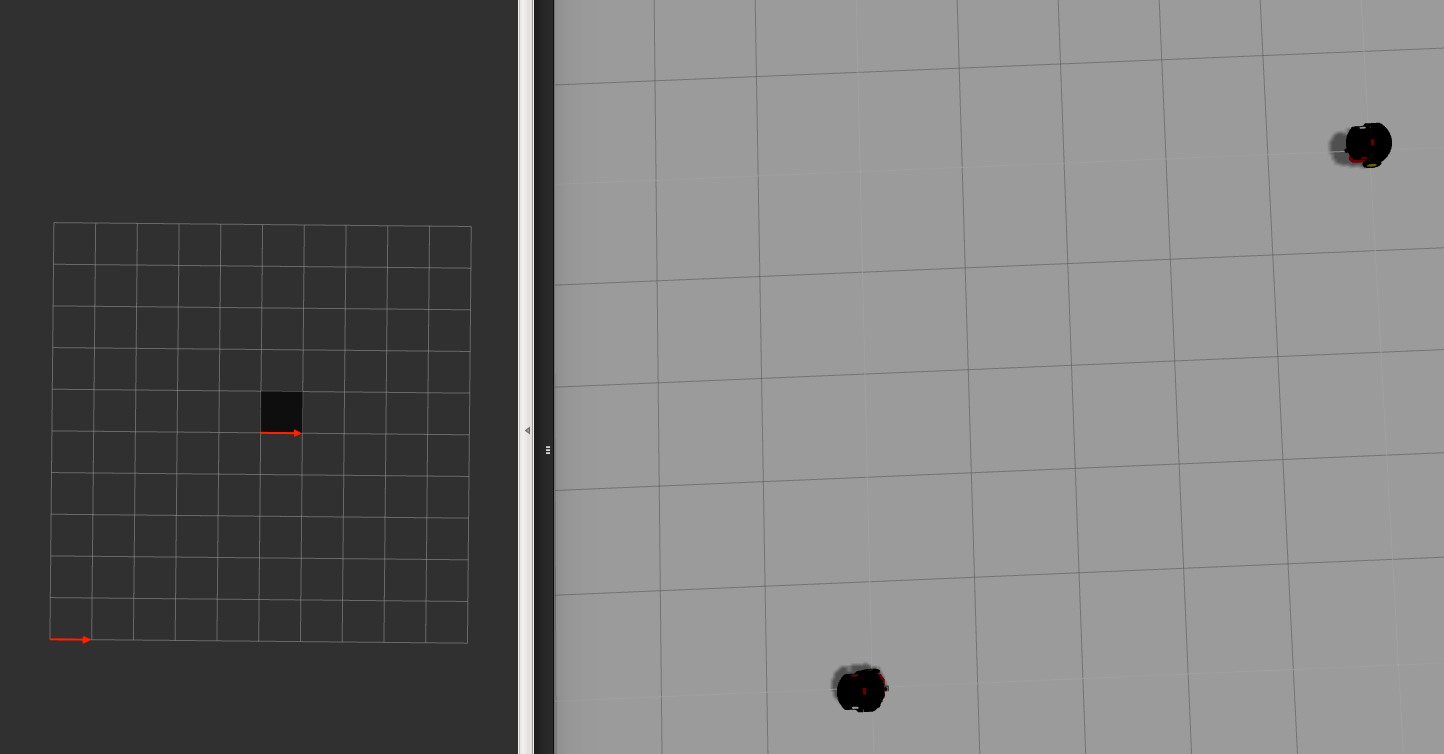
\includegraphics[height=4cm]{figs/simulation_environment_.png}
  \caption{Gazebo simulation environment. The robot and the target are simulated as differential drive Pioneer 3DX robots.}
  \label{Gazebo}
\end{figure}

\begin{figure}[H]
  \centering
  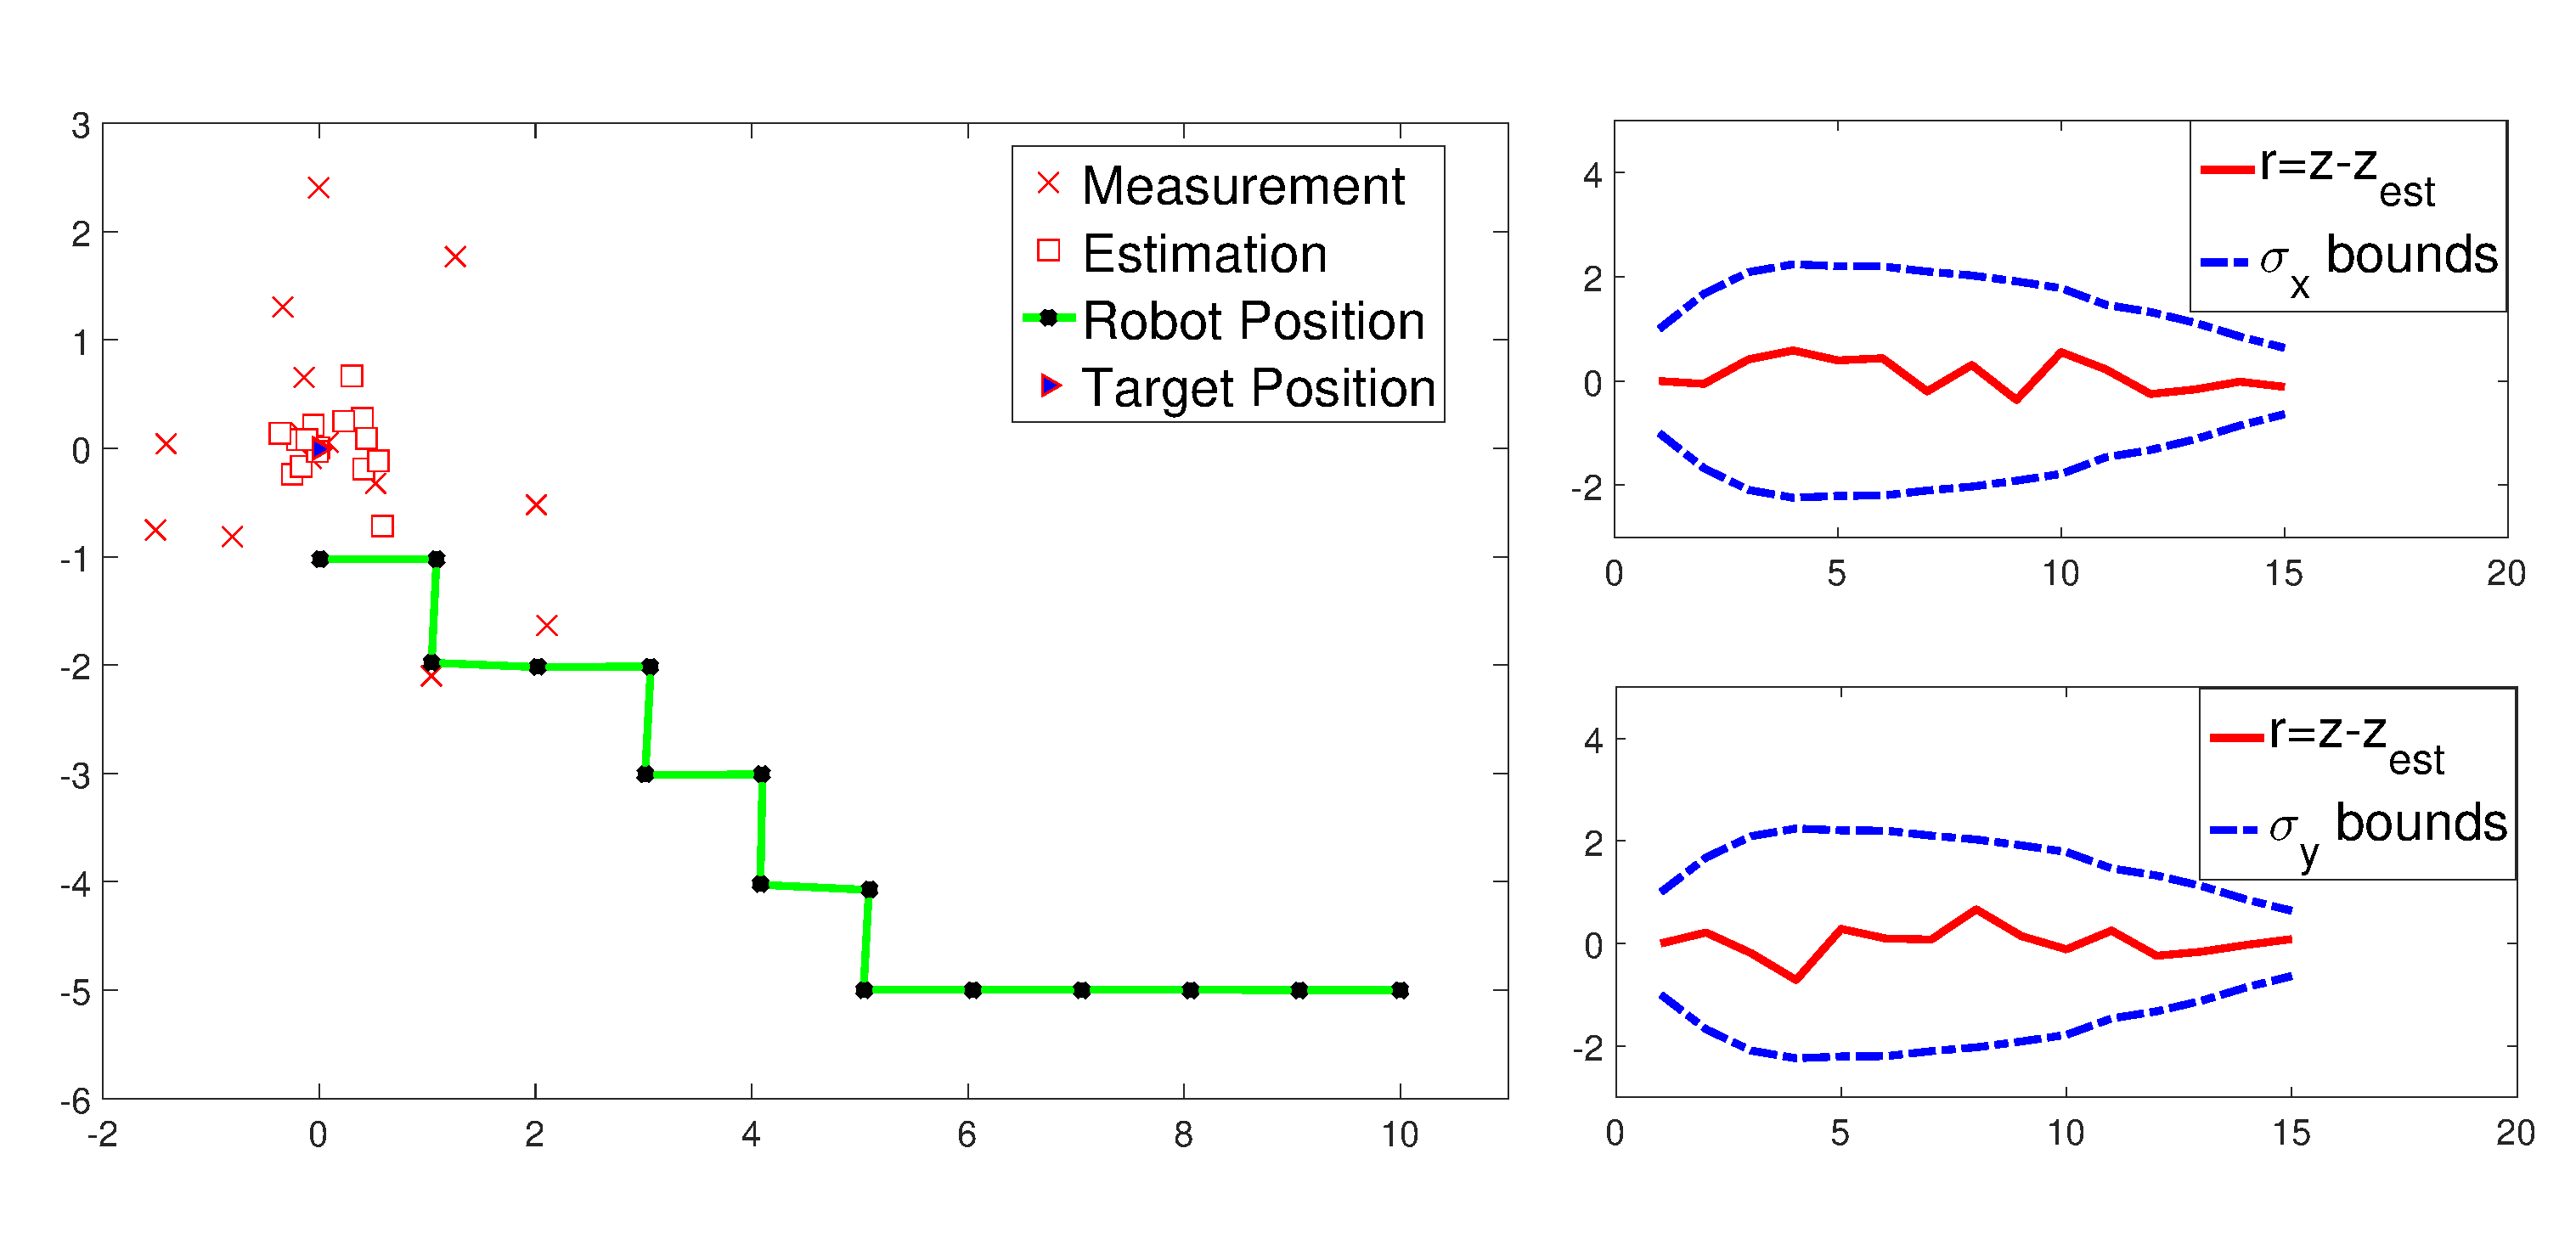
\includegraphics[width=8.5cm]{figs/3_stationary.eps}
  \caption{Tracking a stationary target.}
  \label{online1}
\end{figure}

\begin{figure}[H]
  \centering
  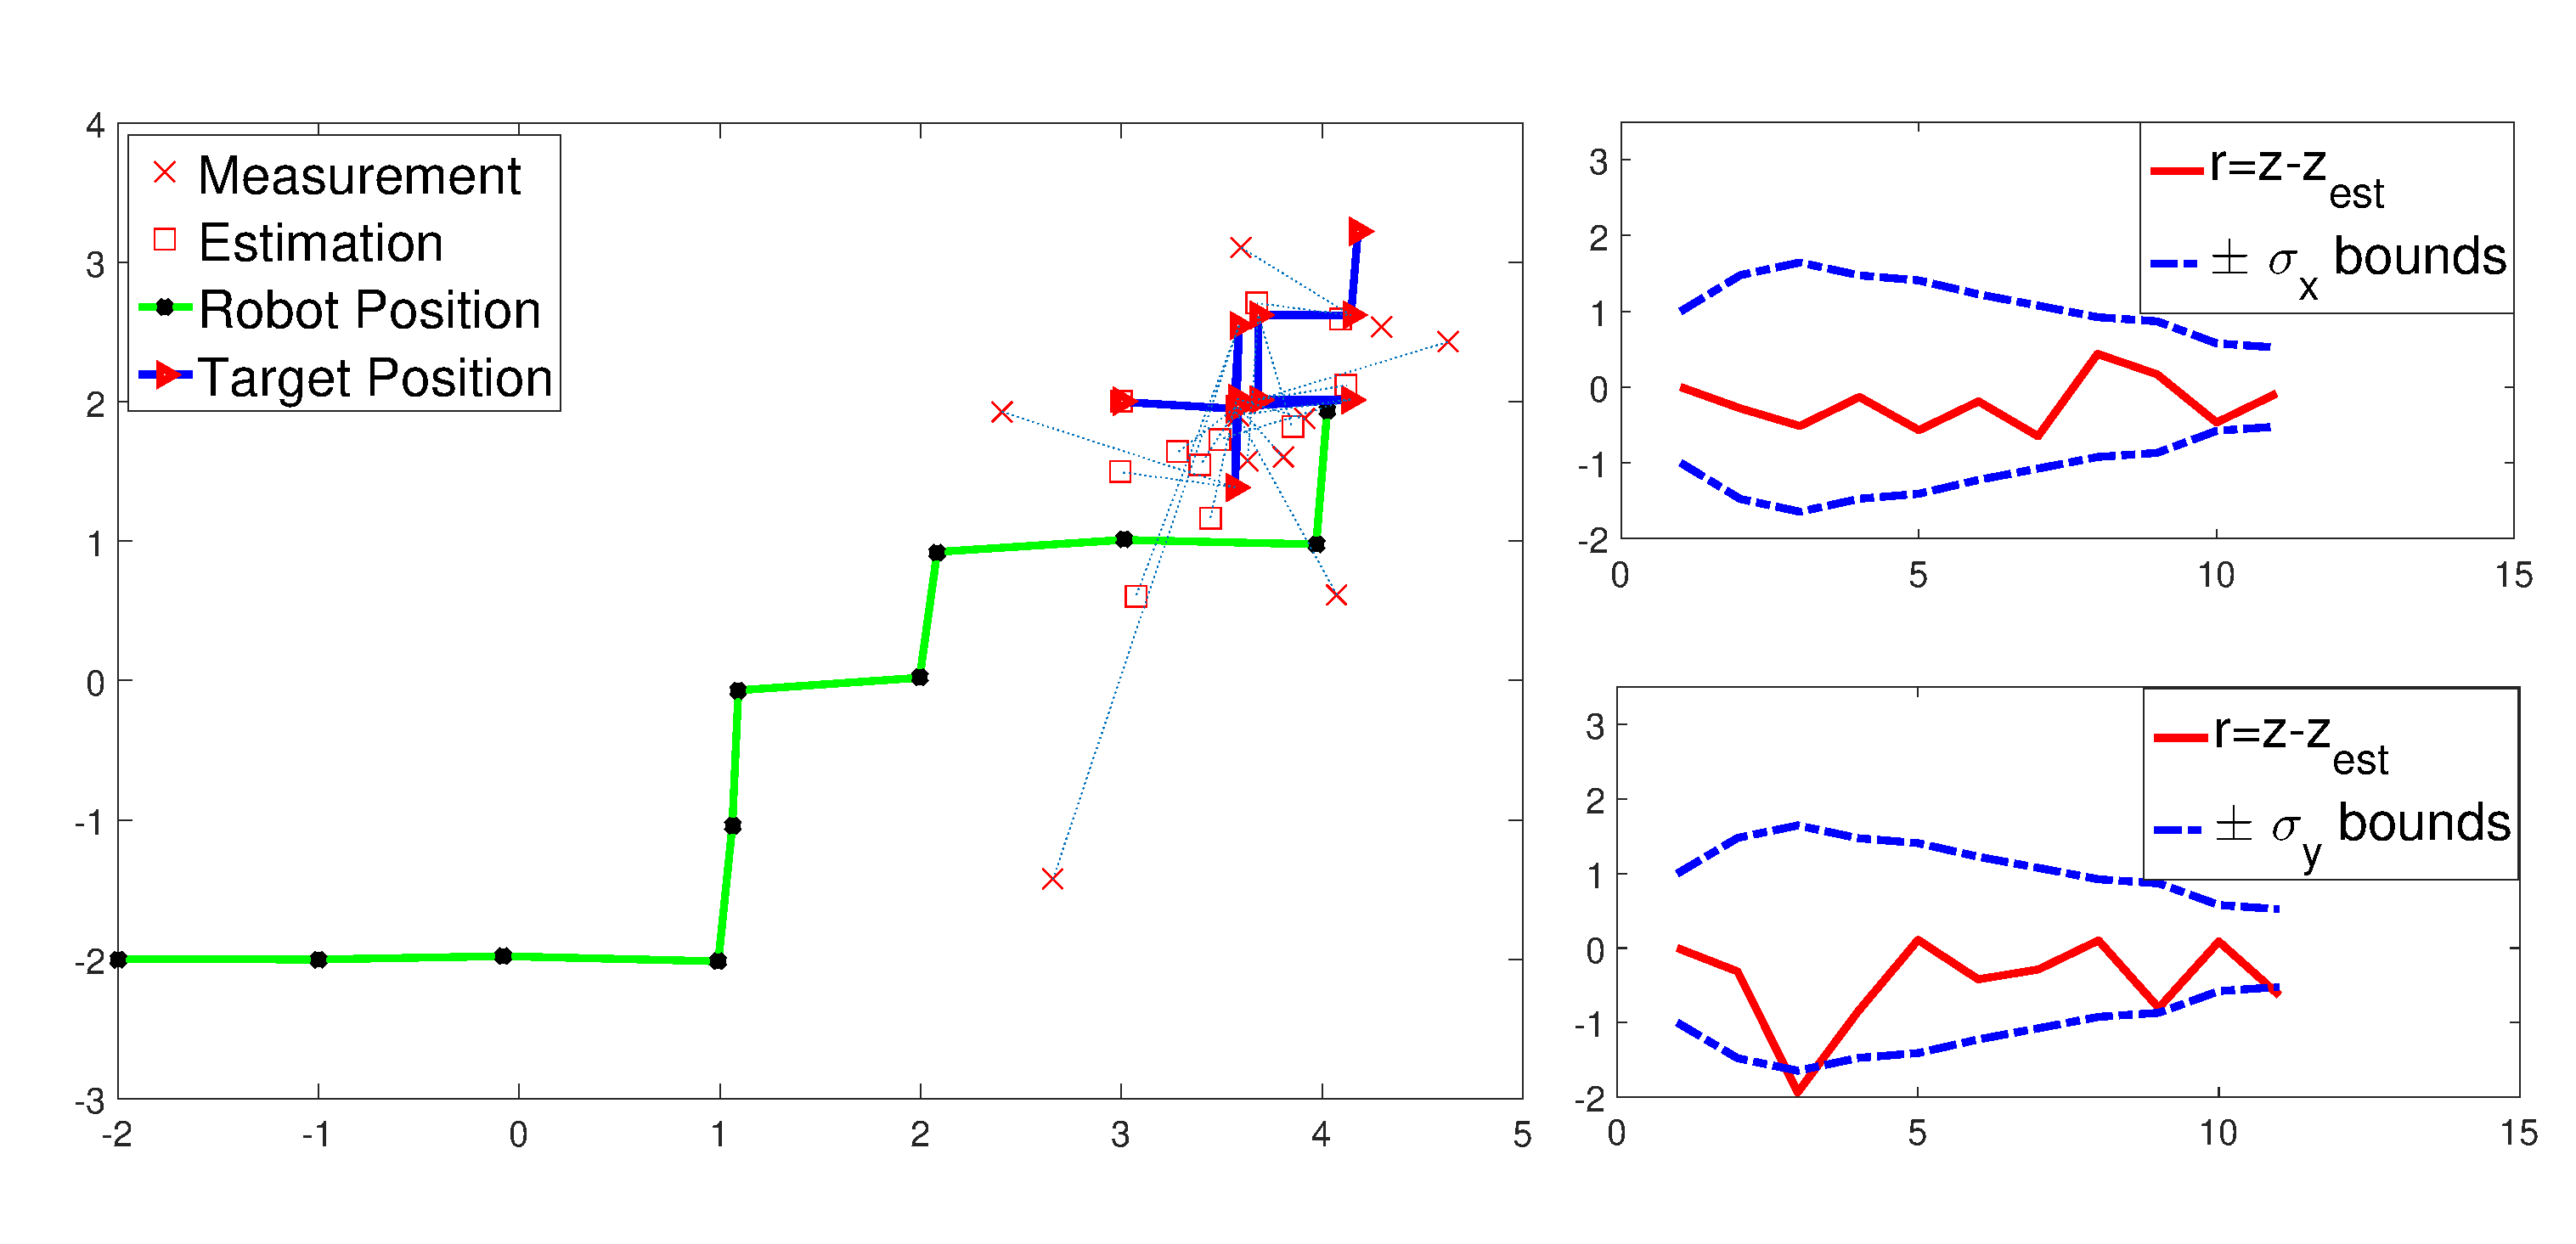
\includegraphics[width=8.5cm]{figs/2_random_walk.eps}
  \caption{Tracking a target that moves with random control inputs.}
  \label{online2}
\end{figure}

\begin{figure}
  \centering
  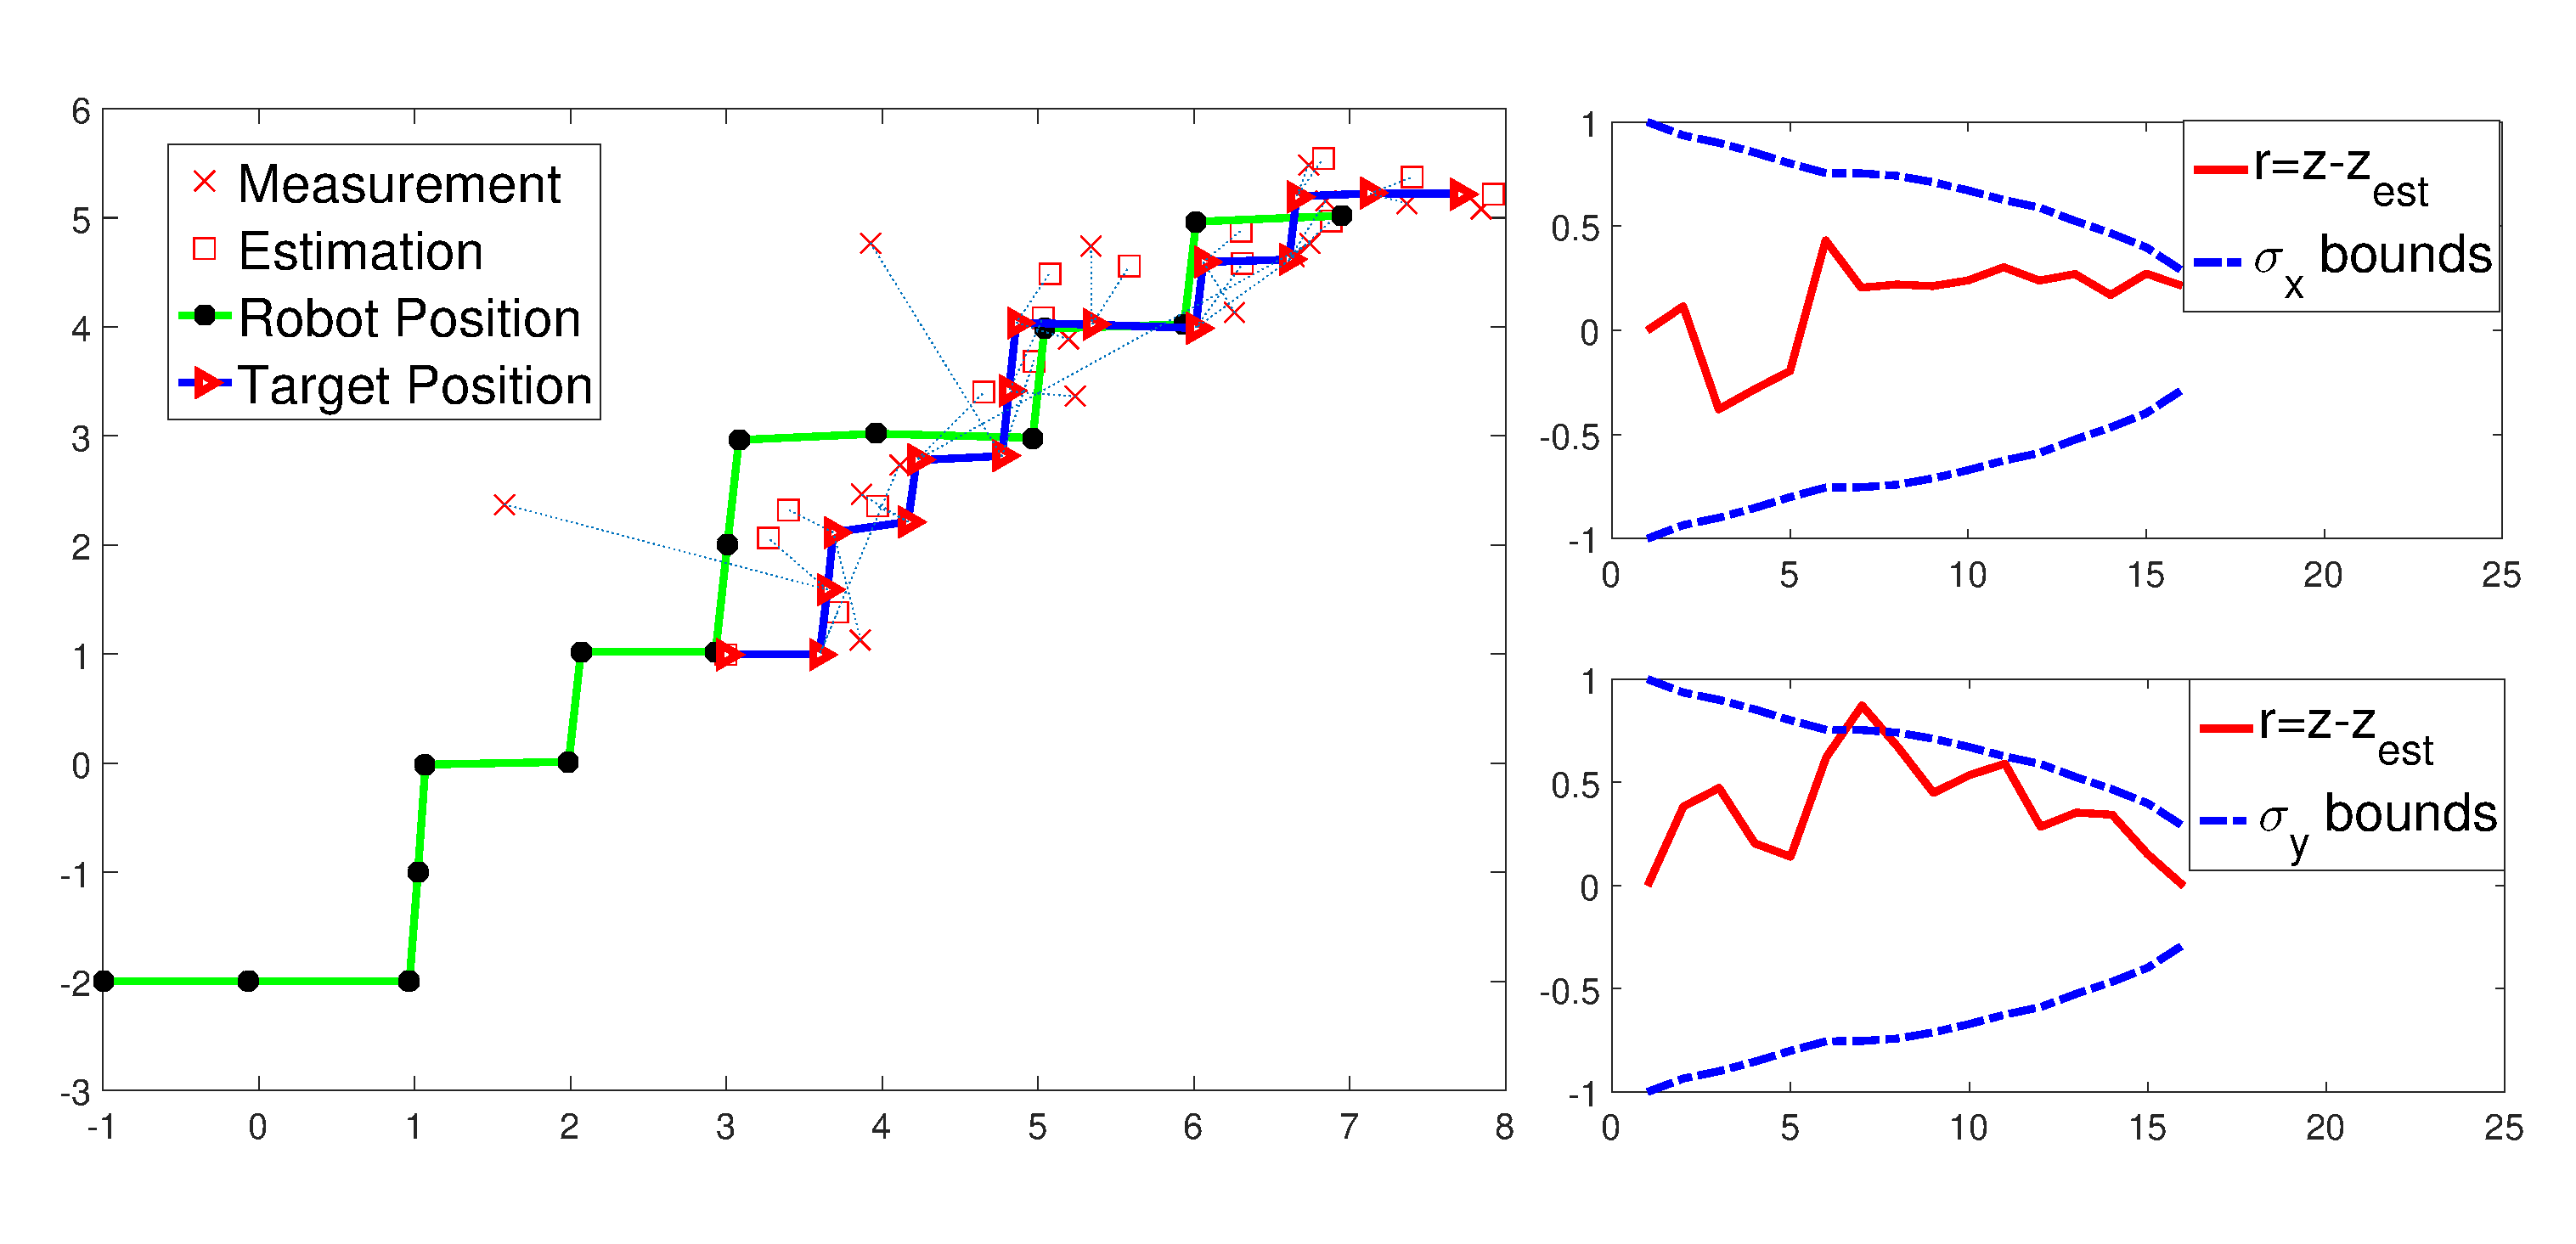
\includegraphics[width=8.5cm]{figs/1_adversary_walk.eps}
  \caption{Tracking a target that actively chooses adversarial control inputs.}
  \label{case3}
\end{figure}


%%%%%%%%%%%%%%%%%%%%%%%%%%%%%%%%%%%%%%%%%%%%%%%%%%%%%%%%%%%%%%%%%%%%%%%%%%%%%%%%
\section{Experiments} 
\label{sec:expt}

We implemented the worst-case minimax tracking algorithm using indoor and outdoor robots. We use a five-level minimax tree with a look-ahead of two steps. Our experiments show that the algorithm can be successfully implemented and executed on real hardware.

For the indoor experiment, we used two Pioneer 3DX robots (Figure~\ref{fig:indoorexpts}). One Pioneer acts as the target and the other acts as the tracking robot. The motion and measurement models and parameters are similar to the Gazebo simulation reported in the previous section. The measurement noise is generated using parameters $\delta_1 = 0.5$ and $\delta_2 = 0.1$ from the true position of the target robot. The robot's speed is $0.4m/s$ and the target's speed is $0.25m/s$. We carried out three sets of experiments: (1) tracking a stationary target; (2) tracking a target that moves in a straight line; and (3) tracking a target that actively chooses adversarial control inputs to evade the tracker. Figure~\ref{fig:indoorexpts} shows the robot and the target's trajectories for the three experiments. In all cases, we see that the minimax algorithm with pruning drives the robot towards the target. Furthermore, the hardware experiments demonstrate that the minimax algorithm can be applied in real-time on actual hardware. Videos from the experiments are reported in the accompanying multimedia file.

\begin{figure}
\centering{
\subfigure[Experimental environment]{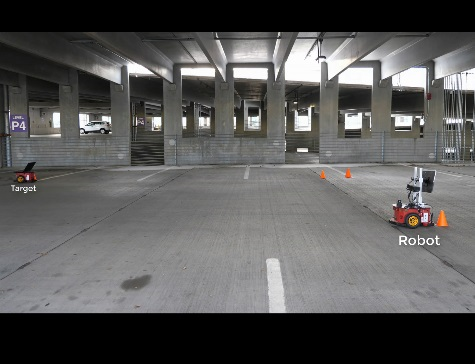
\includegraphics[width=0.43\columnwidth]{figs/snapshot_PioneerTracking.png}}
\subfigure[Tracking a stationary target]{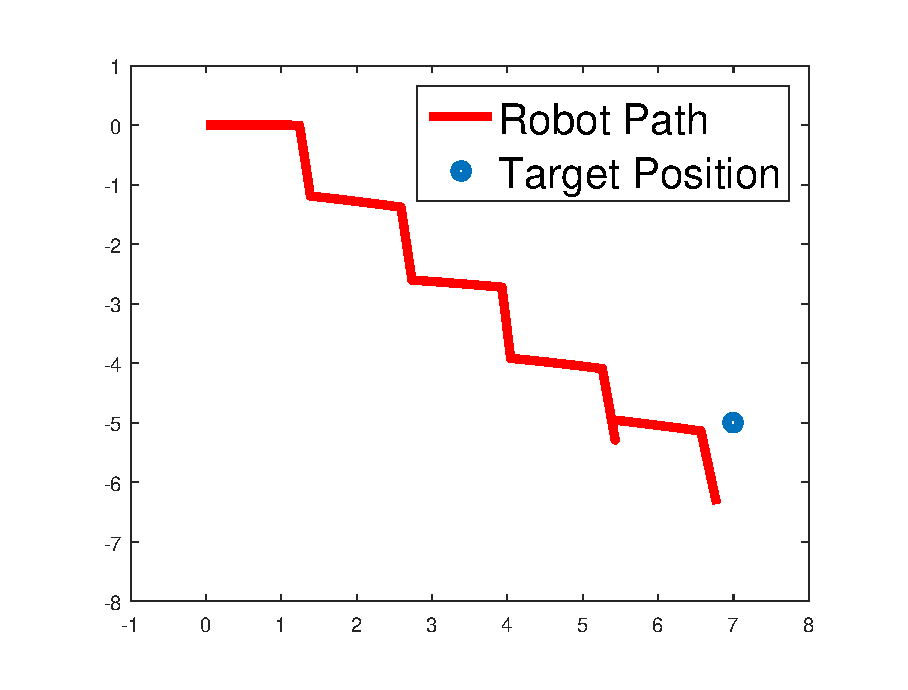
\includegraphics[width=0.47\columnwidth]{figs/Experiment_stationary.eps}}
\subfigure[Tracking a moving target]{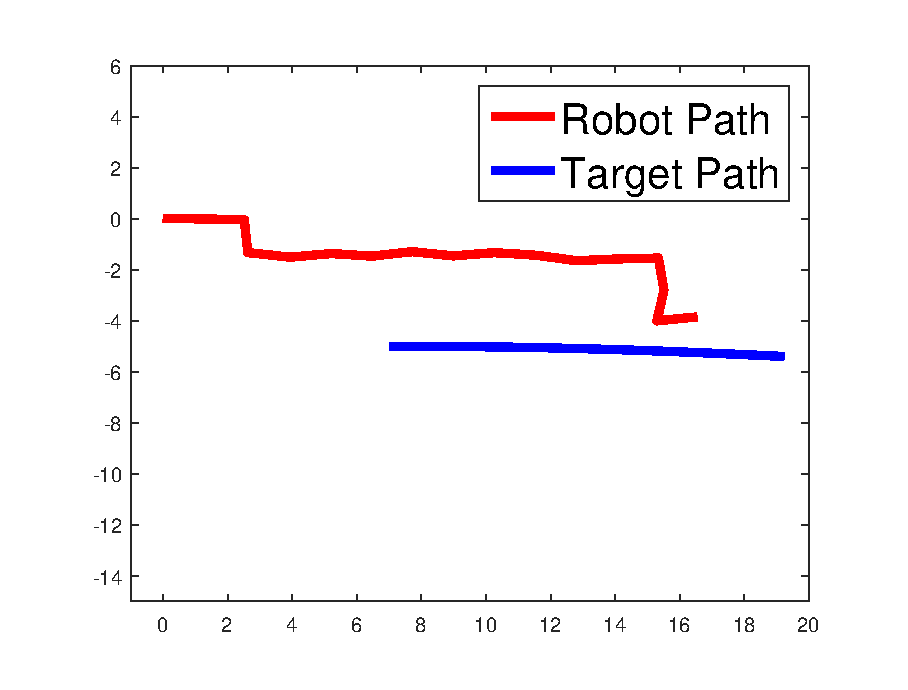
\includegraphics[width=0.47\columnwidth]{figs/Experiment_StraightLine.eps}}
\subfigure[Tracking an adversarial target]{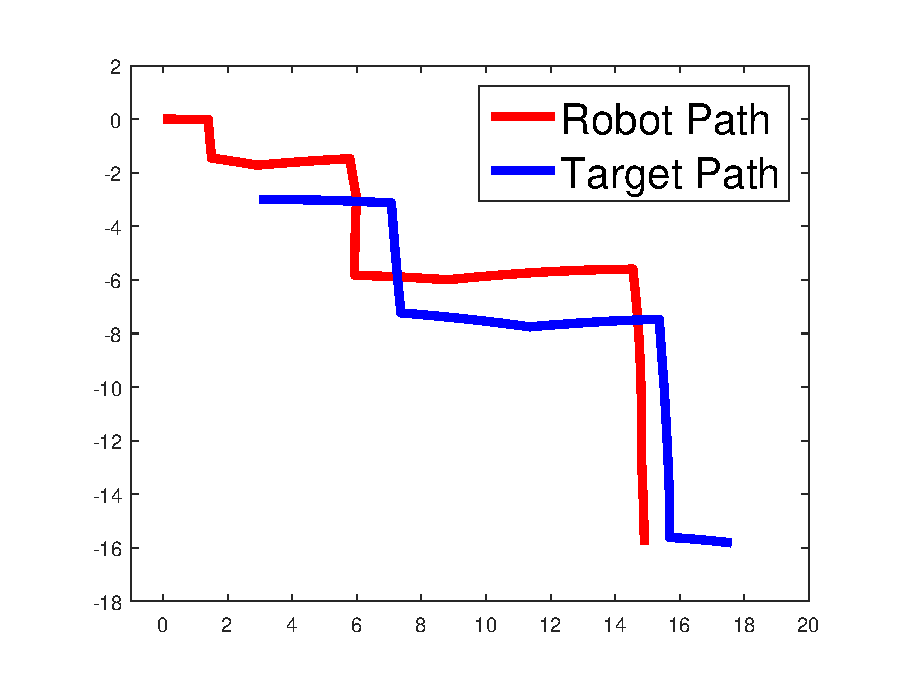
\includegraphics[width=0.47\columnwidth]{figs/Experiment_Adversarial.eps}}
}
\caption{Real-world indoor tracking experiments.}
\label{fig:indoorexpts}         
\end{figure}


\begin{figure}
\centering{
\subfigure[Experimental environment]{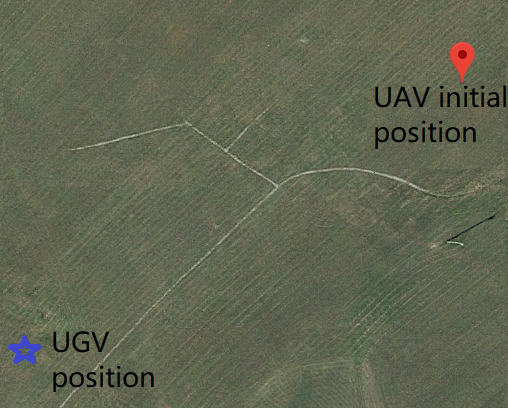
\includegraphics[width=0.43\columnwidth]{figs/Environment_UGVTracking.png}}
\subfigure[UAV online tracking]{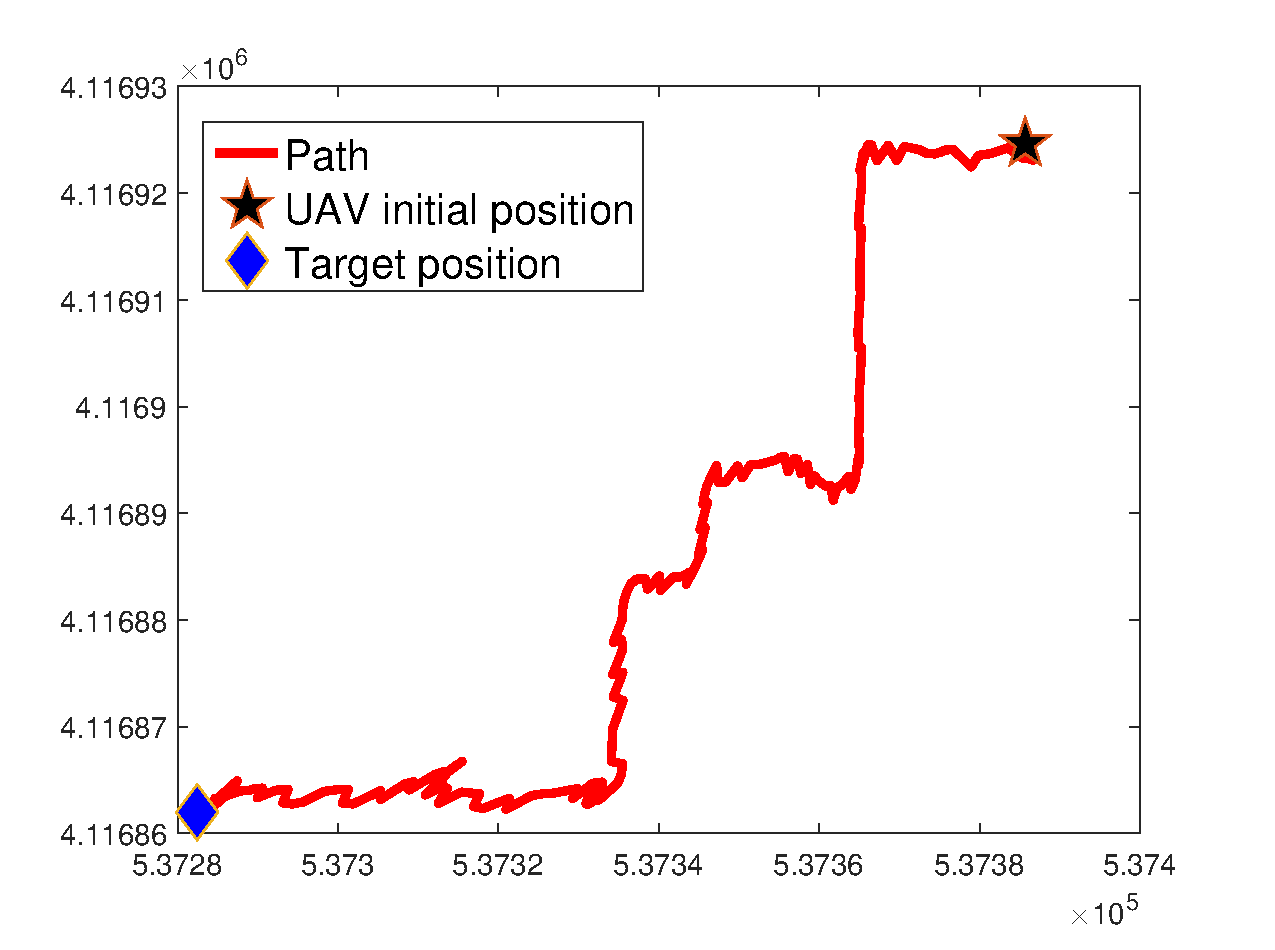
\includegraphics[width=0.47\columnwidth]{figs/Experiment_UAV.eps}}
}
\caption{Real-world outdoor tracking experiment.}
\label{fig:outdoorexpts}         
\end{figure}

The outdoor experiment consisted of an Unmanned Aerial Vehicle (UAV) tracking a stationary target using the minimax tree. The experiments were conducted in a farmland near Blacksburg, VA, USA. The measurement is obtained by a noisy GPS sensor placed on the target. In order to generate the tree, the GPS noise is modeled as a zero mean Gaussian noise with constant variance ($\delta_1 = 0.5$ and $\delta_2 = 0$). The starting position of the UAV was about 160 meters from the target.

The UAV took off manually and then switched to the autonomous mode, where it follows the control commands given by the minimax tree. Figure~\ref{fig:outdoorexpts} shows the resultant trajectory of the UAV produced by the algorithm. Similar to the indoor experiment, the UAV has four motion control input (forward, backward, left, right). The unit step of the UAV is set as 10 meters. The accompanying multimedia attachment contains a video of the outdoor experiment.

The indoor and the outdoor experiments demonstrate that the online minimax tracking algorithm along with the pruning strategy can be applied in real-time on actual hardware.
%%%%%%%%%%%%%%%%%%%%%%%%%%%%%%%%%%%%%%%%%%%%%%%%%%%%%%%%%%%%%%%%%%%%%%%%%%%%%%%


\section{Conclusion}\label{sec:conc}
We investigated the problem of devising closed-loop control policies for target tracking with state-dependent measurement noise. Unlike the state-independent noise case, the value of a candidate control law in our version is a function of the history of measurements obtained. Consequently, planning over a horizon requires taking into account all possible measurement values. 
%A naive strategy is to enumerate all possible future measurements and evaluate all possible sequences of control laws. Even then, since the actual measurements are unknown, we can only minimize the expected or worst-case uncertainty in the target's estimate. 
We focused on minimizing the worst-case uncertainty. Our solution consists of building a minimax search tree to obtain the control policy. A full enumeration tree has a size that is exponential in the number of measurements, control actions, and the planning horizon. Instead, we exploited the structural properties of EKF to yield a tree with significantly less number of possible nodes without sacrificing the optimality guarantees. We also showed how two parameters, $\epsilon_1$ and $\epsilon_2$, can be used to yield even more computational savings at the expense of optimality. The resulting algorithm was evaluated in simulations and through real-world experiments.
%We also presented bounds on the solution sub-optimality as a function of $\epsilon_1$ and $\epsilon_2$. With this, we advance the state-of-the-art by generalizing the best-known algorithms for linear target tracking~\cite{vitus2012efficient, atanasov2014information} to non-linear scenarios.

One disadvantage of the generalization is that we have to discretize the set of possible future measurements. Our immediate future work is to bound the suboptimality as a function of the number of discrete samples chosen to represent the continuous set of  measurements. The second avenue of future work focuses on extending these results to multi-robot, multi-target scenarios. Our prior work~\cite{tokekar2014multi,sung2018distributed} has shown a greedy assignment of robot trajectories to targets yield provably approximate solutions for one-step planning. We will extend this to planning over a finite horizon using the results presented in this paper.





% if have a single appendix:
%\appendix[Proof of the Zonklar Equations]
% or
%\appendix  % for no appendix heading
% do not use \section anymore after \appendix, only \section*
% is possibly needed

% use appendices with more than one appendix
% then use \section to start each appendix
% you must declare a \section before using any
% \subsection or using \label (\appendices by itself
% starts a section numbered zero.)
%


\appendices
\section{Proof of Lemma~\ref{lemma:mono}}
\begin{proof}
For nodes $A$ and $B$ at the same level $k$ with $H\Sigma_{t}^AH^T+S^A \succeq H\Sigma_{t}^BH^T+ S^B$, our goal is to prove that $\rho(\Sigma_{t}^A)\succeq \rho(\Sigma_{t}^B)$.

Applying the Riccati equation we have:
\begin{equation}
\begin{split}
&\rho(\Sigma_{t}^A)- \rho(\Sigma_{t}^B)\\
=&C_t\Sigma_{t}^AC_t^T-C_t\Sigma_{t}^AH^T\left(H\Sigma_{t}^AH^T+S^A\right)^{-1}H\Sigma_{t}^AC_t^T\\
&-  C_t\Sigma_{t}^BC_t^T+C_t\Sigma_{t}^BH^T\left(H\Sigma_{t}^BH^T+ S^B\right)^{-1}H\Sigma_{t}^BC_t^T  
\end{split}
\end{equation}
We define:
\begin{align*}
K(\Sigma_t) &\triangleq -C_t\Sigma_t H^T(H\Sigma_t H^T+S)^{-1}\\
F(\Sigma_t) &\triangleq C_t-(C_t\Sigma_t H_t^T)(H\Sigma_t H^T+S)^{-1}H
\end{align*}
Note that:
\begin{align*}
F(\Sigma_t) &= C_t+K(\Sigma_t)H\\
K(\Sigma_t)(C_t\Sigma_t H^T)^T & =-K(\Sigma_t)(H\Sigma_t H^T+S)K^T(\Sigma_t)
\end{align*}
Then, we have,
\begin{equation}
\begin{split}
\rho&(\Sigma^A_{t})-\rho(\Sigma^B_{t})-F(\Sigma^A_{t})(\Sigma^A_{t}-\Sigma^B_{t})F(\Sigma^A_{t})^T\\
=&C_t\Sigma_t^AC_t^T + K(\Sigma_t^A)H\Sigma_t^AC_t^T \\
&- [C_t\Sigma_t^BC_t^T+ K(\Sigma_t^B)H\Sigma_t^BC_t^T]\\
&- [C_t+K(\Sigma_t^A)H](\Sigma_t^A-\Sigma_t^B)[C_t+K(\Sigma_t^A)H]^T\\
=&K(\Sigma^A_{t})C_t\Sigma^A_{t}H^T-K(\Sigma^B_{t})C_t\Sigma^B_{t}H^T\\
&-K(\Sigma^A_{t})H(\Sigma^A_{t}-\Sigma^B_{t})C_t^T-C_t(\Sigma^A_{t}-\Sigma^B_{t})H^TK^T(\Sigma^A_{t})\\
&-K(\Sigma^A_{t})H(\Sigma^A_{t}-\Sigma^B_{t})H^TK^T(\Sigma^A_{t})\\
=&K(\Sigma^A_{t})C_t\Sigma^A_{t}H^T-K(\Sigma^B_{t})C_t\Sigma^B_{t}H^T\\
&-K(\Sigma^A_{t})[H\Sigma^A_{t}C_t^T-H\Sigma^B_{t}C_t^T]\\
&-[C_t\Sigma^A_{t}H^T-C_t\Sigma^B_{t}H^T]K^T(\Sigma^A_{t})\\
&-K(\Sigma^A_{t})H(\Sigma^A_{t}-\Sigma^B_{t})H^TK^T(\Sigma^A_{t})\\
=&-K(\Sigma^B_{t})(C_t\Sigma^B_{t}H^T)+K(\Sigma^A_{t})(C_t\Sigma^B_{t}H^T)\\
&+(C_t\Sigma^B_{t}H^T)K^T(\Sigma^A_{t})\\
&+K(\Sigma^A_{t})(H\Sigma^B_{t}H^T+S^A)K^T(\Sigma^A_{t})\\
=&K(\Sigma^B_{t})(H\Sigma^B_{t}H^T+S^B)K^T(\Sigma^B_{t})\\
&+K(\Sigma^A_{t})(H\Sigma^B_{t}H^T+S^A)K^T(\Sigma^A_{t})\\
&-K(\Sigma^A_{t})(H\Sigma^B_{t}H^T+S^B)K^T(\Sigma^B_{t})\\
&-K(\Sigma^B_{t})(H\Sigma^B_{t}H^T+S^B)K^T(\Sigma^A_{t})\\
=&(K(\Sigma^B_{t})-K(\Sigma^A_{t}))(H\Sigma^B_{t}H^T+S^B)(K(\Sigma^B_{t})-K^T(\Sigma^A_{t}))\\
&+K(\Sigma^A_{t})(S^A-S^B)K^T(\Sigma^A_{t})
\end{split}
\end{equation}
Define\footnote{Here,  $C=\min(A,B)$ implies $C = A$ if $B - A \succeq 0$, otherwise $C = B$.}, 
\begin{equation}\label{maxM}
\begin{split}
P_t P^T_t=\min((&C_tH^{-1}+K(\Sigma^A_{t})H)(C_tH^{-1}+K(\Sigma^A_{t})H)^T, \\ &K(\Sigma^A_{t})K^T(\Sigma^A_{t}) )
\end{split}
\end{equation}
So, we have,
\begin{equation}
\begin{split}
&\rho(\Sigma^A_{t})-\rho(\Sigma^B_{t})\\
=&F(\Sigma^A_{t})(\Sigma^A_{t}-\Sigma^B_{t})F^T(\Sigma^A_{t})+K(\Sigma^A_{t})(S^A-S^B)K^T(\Sigma^A_{t})\\
&+(K(\Sigma^B_{t})-K(\Sigma^A_{t}))(H\Sigma^B_{t}H^T+S^B)\cdot\\
&\quad(K(\Sigma^B_{t})-K(\Sigma^A_{t}))^T\\
=&(C_t+K(\Sigma^A_{t})H)(\Sigma^A_{t}-\Sigma^B_{t})(C_t+K(\Sigma^A_{t})H)^T\\
&+K(\Sigma^A_{t})(S^A-S^B)K^T(\Sigma^A_{t})\\
&+(K(\Sigma^B_{t})-K(\Sigma^A_{t}))(H\Sigma^B_{t}H^T+S^B)\cdot\\
&\quad(K(\Sigma^B_{t})-K^T(\Sigma^A_{t}))\\
&\text{From [\ref{maxM}], we have}\\
\succeq & P_t H(\Sigma^A_{t}-\Sigma^B_{t})H^T  P^T_t\\
&+P_t (S^A-S^B) P^T_t\\
&+(K(\Sigma^B_{t})-K(\Sigma^A_{t}))(H\Sigma^B_{t}H^T+S^B)\cdot\\
&\quad(K(\Sigma^B_{t})-K(\Sigma^A_{t}))^T\\
= & P_t \left((H\Sigma^A_{t}H^T+S^A)-(H\Sigma^B_{t}H^T+S^B)\right) P^T_t\\
&+(K(\Sigma^B_{t})-K(\Sigma^A_{t}))(H\Sigma^B_{t}H^T+S^B)\cdot\\
&\quad(K(\Sigma^B_{t})-K(\Sigma^A_{t}))^T
\end{split}
\label{inequaility}
\end{equation}
Since $H\Sigma_{t}^AH^T+S^A \succeq H\Sigma_{t}^BH^T+ S^B$, we have
\begin{equation}
\rho(\Sigma^A_{t})-\rho(\Sigma^B_{t}) \succeq 0
\end{equation}
\end{proof}
% you can choose not to have a title for an appendix
% if you want by leaving the argument blank

\section{Proof of Theorem~\ref{thm:main}}
\begin{proof}
We first prove a special case when $\mathcal{H}$ consists of only one node, $B$. That is, we have:
\begin{equation*}
H\Sigma_t^AH^T \succeq H\Sigma_t^BH^T+M\cdot aI
\end{equation*}
where, $a=\delta_1^2 +\delta_2^2\mathcal{C}$. We want to prove the following:
\begin{equation}
\text{tr}(\Sigma_{t+M}^A) \ge \text{tr}(\Sigma^B_{t+M}).
\label{eqn:singleH}
\end{equation}

We will prove this by induction. We start with the base case.

\noindent\textbf{Base step:} Show that Equation~\ref{eqn:singleH} holds for $M = 1$.

When $M = 1$, $H\Sigma^A_{t}H^T \succeq H\Sigma^B_tH^T+aI$. From the Kalman filter Riccati map,
\begin{equation}
\begin{split}
&\Sigma^A_{t+1}=\rho_i(\Sigma^A_{t})\\
=&C_t\Sigma^A_{t}C_t^T-C_t\Sigma^A_{t}H^T\cdot\\
&\left(H\Sigma^A_{t}H^T+\Sigma_{w_i}\left(x_r(t),\hat{x}^A_o(t)\right)\right)^{-1}H\Sigma^A_{t}C_t^T+\Sigma_v
\end{split}
\end{equation}
Applying Lemma~\ref{lemma:mono}, we get,
\begin{equation}
\begin{split}
&\Sigma^A_{t+1}\\
\succeq& C_t\Sigma^B_{t}C^T-C_t\Sigma^B_{t}H^T\cdot\\
&\left(H\Sigma^B_{t}H^T+\Sigma_{w_i}\left(x_r(t),\hat{x}^B_o(t)\right)\right)^{-1}H\Sigma^B_{t}C_t^T+\Sigma_v\\
=&\Sigma^B_{t+1}
\end{split}
\end{equation}

\noindent\textbf{Inductive step:} Show that if Equation~\ref{eqn:singleH} holds for $M=k$, then it also holds for $M=k+1$. This can be done as follows:
\begin{equation*}
H\Sigma_t^AH^T \succeq H\Sigma_t^BH^T+(k+1)\cdot aI
\end{equation*}
Rewrite the equation as:
\begin{equation*}
H_t\Sigma_t^AH_t^T \succeq H_t[\Sigma_t^B+a\cdot(H^TH)^{-1}]H_t^T+k\cdot aI
\end{equation*}
Since $M=k$ holds for some $k$. Let $\Sigma^{B'}_{t}=\Sigma^B_{t}+a\cdot (H^TH)^{-1}$, based on the condition of $M=k$ we have,
$$\Sigma^A_{t+k} \succeq \Sigma^{B'}_{t+k}$$
that is,
$$\Sigma^A_{t+k} \succeq \Sigma^B_{t+k}+a\cdot (H^TH)^{-1}$$
Similar to the base step:
$$\Sigma^A_{t+k+1} \succeq \Sigma^B_{t+k+1}$$
Thereby showing that indeed $M=k+1$ holds.

Therefore, by mathematical induction, Equation~\ref{eqn:singleH} holds for all integers $M$. Next, we extend this result from $|\mathcal{H}| = 1$ to $ N$ comparable nodes in $\mathcal{H}$. Our goal is to prove the following:
\begin{equation}
\begin{aligned}
\text{tr}&\left(  H\left( \Sigma^A_{t}\right) H^T \right) \ge \\  &\qquad \quad \sum^{i=N}_{i=1}\alpha_i\text{tr}\left( \left[H\Sigma^i_{t}H^T+K\cdot aI\right] \right)
\end{aligned}
\label{eqn:multiH}
\end{equation}
Without loss of generality, we assume $\Sigma^B$ is the minimum covariance matrix among  $\Sigma^1_{t},\Sigma^2_{t},...,\Sigma^N_{t}$. We have:
\begin{equation}
\begin{split}
&\sum^{i=N}_{i=1} \alpha_i \left(\left[H\Sigma^i_{t}H^T+N\cdot aI\right])\right)\\
&\qquad\succeq \sum^{i=N}_{i=1} \alpha_i \left(\left[H\Sigma^B_{t}H^T+N\cdot aI\right]\right)\\
&\qquad = H\Sigma^B_{t}H^T+N
\cdot aI
\end{split}
\end{equation}
So, 
\begin{equation}
\text{tr}\left(  H\left( \Sigma^A_{t}\right) H^T \right) \ge   \text{tr}\left(H\Sigma^B_{t}H^T+K\cdot aI\right)
\end{equation}
This conditions says that the trace of the covariance at node $A$ is greater than the trace of covariance of any successor of node $B$ for a tree of depth at most $K$. Therefore, node $A$ will not be part of the optimal policy and can be pruned without affecting optimality of the minimax tree.
\end{proof}

\section{Proof of Theorem~\ref{thm:epsilon2bound}}
\begin{proof}
For some level $i$, suppose that we prune a node on the optimal policy. We have,
$$\text{tr}(H\left(\Sigma_{2i}^{\epsilon_2}\right) H^T) \le \text{tr}(H\left(\Sigma_{2i}^{*}+\epsilon_2I\right)H^T)$$ 
From~\cite{vitus2012efficient}, we know that $\forall\Sigma, Q \in \mathbb{R}^{n\times n}$ and $\epsilon \geq 0$:
$$\rho_{2i}(\Sigma+\epsilon Q)\preceq \rho_{2i}(\Sigma) + F_i(\Sigma)QF^T_i(\Sigma)\epsilon.$$

Applying to the above equation we get, 
\begin{align*}
\Phi_{2k}&(\Sigma+\epsilon_2Q) = \rho_{2(k-1)}(\Phi_{2(k-1)}(\Sigma+\epsilon_2Q))\\
=&\rho_{2(k-1)}(\rho_{2(k-2)}( \dots \rho_0(\Sigma+\epsilon_2Q)))\\
\preceq& \Phi_{2k}(\Sigma)+ \rho_{2(k-1)}(\rho_{2(k-2)}( \dots \rho_2(F_1(\Sigma)QF^T_1(\Sigma))\\
\vdots\\
=&\Phi_{2k}(\Sigma)+\\ &\left[  \prod^0_{i=k-1}\left( F_i(\Sigma) \Phi_{2i}(\Sigma)\right) Q  \prod^{k-1}_{i=0}\left(  F_i(\Sigma) \Phi_{2i}(\Sigma)\right)^T \right]\epsilon_2\\ &+o(\epsilon_2)\\
\preceq &\Phi_{2k}(\Sigma)+\\ &\left[  \prod^0_{i=k-1}\left( F_i(\Sigma) \Phi_{2i}(\Sigma)\right) Q  \prod^{k-1}_{i=0}\left(  F_i(\Sigma) \Phi_{2i}(\Sigma)\right)^T \right]\epsilon_2
\end{align*}

Let $\left\lbrace \hat{\Sigma}^\ast_i\right\rbrace^k_{i=1} $ be the series of covariance matrices along the optimal minimax trajectory. Suppose that the sequence of covariace matrices along the optimal trajectory returned by $\epsilon_2$--algebraic redundancy pruning algorithm  is  $\left\lbrace \hat{\Sigma}^{\epsilon_2}_i\right\rbrace^k_{i=1} $. We get,
$$\hat{\Sigma}^{\epsilon_2}_i \preceq \hat{\Sigma}^{\ast}_i+\epsilon_2I,\quad \forall i=1,2,\dots,k$$ 

By combining the two results, we obtain the desired bound:
\begin{align*}
&0\leq  J_{2k}^{\epsilon_2}-J_{2k}^\ast = \Tr(\hat{\Sigma}^{\epsilon_2}_k)-\Tr(\hat{\Sigma}^{\ast}_k)\\
& \leq \Tr\left\{  \sum^k_{j=0} \left[ \prod^j_{i=k-1}\left( F_i(\Sigma) \Phi_{2i}(\Sigma)\right) \prod^{k-1}_{i=j}\left(  F_i(\Sigma) \Phi_{2i}(\Sigma)\right)^T \right]\epsilon_2 
\right\} \\
&=B^{\epsilon_2}
\end{align*}
\end{proof}

% use section* for acknowledgment
\section*{Acknowledgment}
The authors would like to thank Lifeng Zhou and Yoonchang Sung for their help with the experiments.


\bibliographystyle{plain}
\bibliography{main,refs}



%\begin{IEEEbiography}{Zhongshun Zhang}
%Biography text here.
%\end{IEEEbiography}
%
%\begin{IEEEbiography}{Pratap Tokekar}
%Biography text here.
%\end{IEEEbiography}

\end{document}


